% James Gardner, ASC2 semester 2, 2019
\documentclass[12pt,a4paper]{article}
\usepackage[utf8]{inputenc}
\usepackage{amsmath,amssymb,amsthm}
\usepackage{graphicx}%,subfig}
\usepackage{float}
\usepackage{hyperref}
\usepackage{mathtools}
\usepackage{siunitx}
% \usepackage{float}    
\usepackage{subcaption}
% \usepackage{biblatex}
\usepackage{natbib}
\usepackage{multirow}

\graphicspath{{./pics/}}

\setlength{\parindent}{0pt}
\newcommand\hmmax{0}
\newcommand\bmmax{0}
\newcommand{\norm}[1]{\left\lVert#1\right\rVert}

\title{Blob-match: Machine learning for cross-identification of radio surveys}
\author{James Gardner, supervisors:\ Cheng Soon Ong, Matthew Alger}
\date{Semester 2 2019}

\begin{document}
\maketitle

\begin{abstract}
    % Hey, my name is James and this is my wicked cool report.
    % It sure is!
    \noindent
    Achieving success in radio-radio survey cross-identification would be determining the real, physical objects that we're looking up at. The simplest measure of whether two sources (or `blobs') are a match for an actual object is their separation on the sky. Using this separation, we create a common catalogue of positional matches from the radio surveys TGSS (TIFR GMRT Sky Survey Alternative Data Release 1) and NVSS (NRAO VLA Sky Survey), and reproduce the initial results of \citet{posmatchpaper}. We train a logistic regression binary classifier on half this catalogue, which successfully predicts the positional matching labels on the other half. We then use its predictions to naively partition a patch of the sky into objects, by transitively grouping any chain of predicted matches. This fails to convincingly identify objects in the sky, but we find the core problem to be with positional matching itself.
\end{abstract}

\begin{figure}
    \centering
    \scalebox{-1}[1]{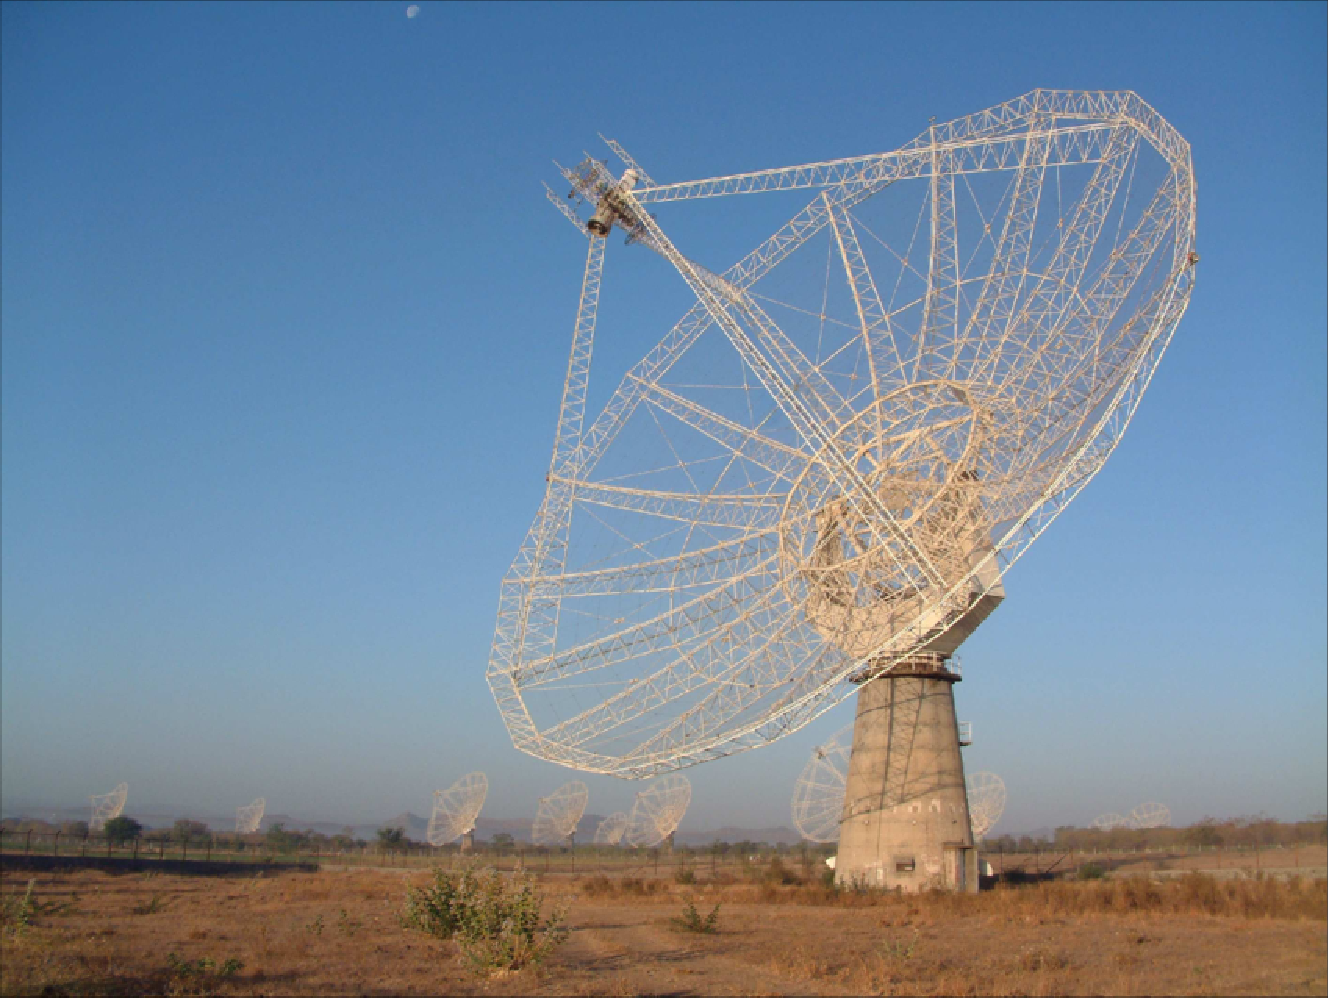
\includegraphics[width=0.44\textwidth]{pics/GMRT.pdf}} \;\;
    \scalebox{-1}[1]{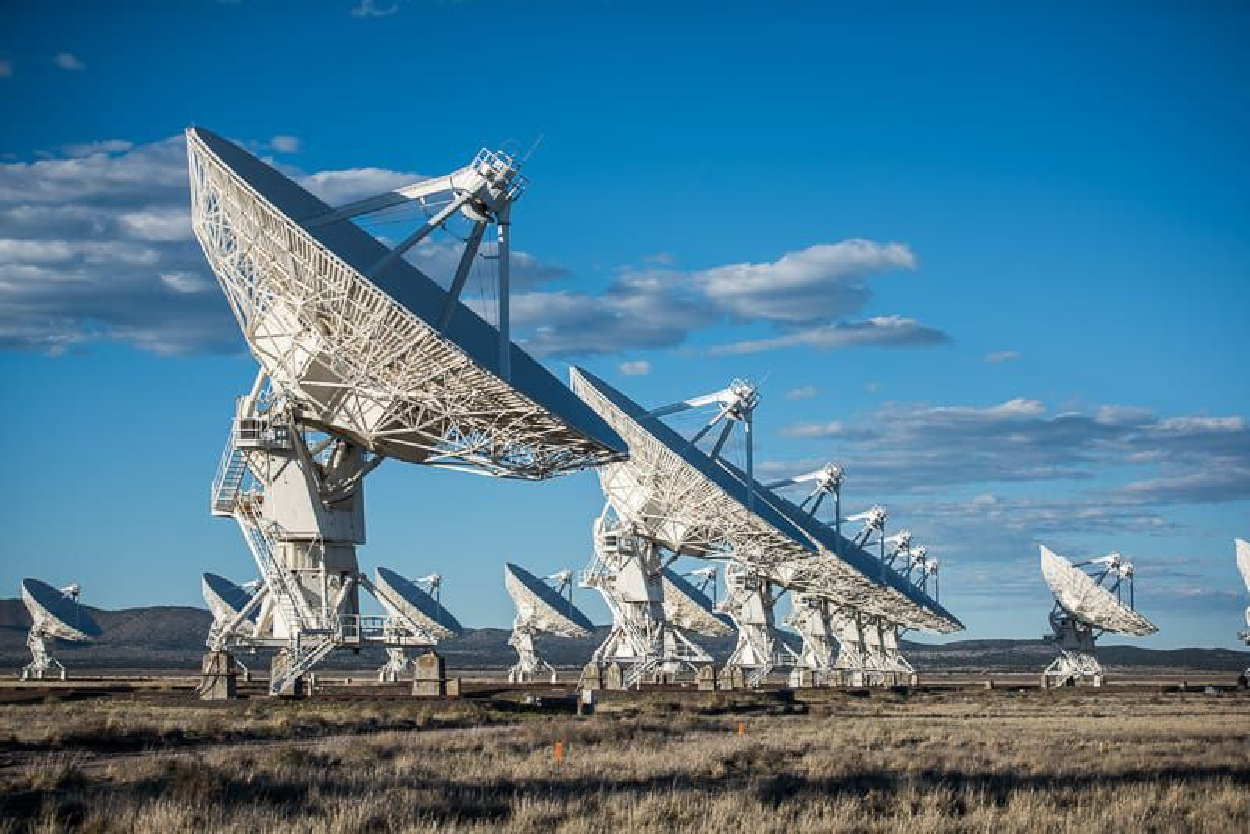
\includegraphics[width=0.5\textwidth]{pics/VLA.pdf}}
    \caption{Giant Metrewave Radio Telescope, (TGSS) at 150 MHz, $\ang{;;25}$ resolution, left; Very Large Array, (NVSS) at 1.4 GHz, $\ang{;;45}$ resolution, right.}
    \label{fig:telescopes}
\end{figure}

\newpage
\section{Introduction}
\label{sec:introduction}
% motivation
What's out there in the universe? This is the central question of astronomy. To determine what physical objects lie out there, we consider the different images seen in two radio sky surveys. We choose to compare surveys because there's extra information encoded in how the objects appear at different frequencies. Being able to combine multiple existing measurements, with different parameters, into one holistic model is valuable in general. But here it is essential to come up with sound methods to compare and combine different views of the sky. In order to make the best informed predictions we can given the limited information we have.\\

For the rest of this chapter~\ref{sec:introduction} we'll present the problem of cross-identification. In chapter~\ref{sec:positional_matching}, we'll address this problem with the method of positional matching, reproducing the initial results of \citet{posmatchpaper} along the way. Finally, in chapter~\ref{sec:logistic_regression}, we'll apply machine learning to automate the classification of matches, then try to use it to identify physical objects in the sky.

\subsection{Cross-identification}
We consider matches between sources in TGSS (TIFR GMRT Sky Survey Alternative Data Release 1) and NVSS (NRAO VLA Sky Survey). A source in each of the surveys is a two-dimensional gaussian (a `blob') fitted over the raw data. To clarify, there are three layers at play:
\begin{itemize}
    \item[(1)] the real physical object that exists out in the universe
    \item[(2)] the raw photometric data detected by each of the Giant Metrewave Radio Telescope (TGSS) and the Very Large Array (NVSS) (see figure~\ref{fig:telescopes})
    \item[(3)] the sources as gaussians that are fit to the plane of raw data
\end{itemize}
Our goal is to go from pairs of these sources (one in each survey) back to the physical objects as best we can. To do this we must overcome the projection of the real, three-dimensional objects down into the two-dimensional images that we observe. And although `object' is a vague term, astrophysically we understand that this means some system with locality, often gravitationally bound.\\

% 3c40 cut-outs
\begin{figure}[H]
    \centering
    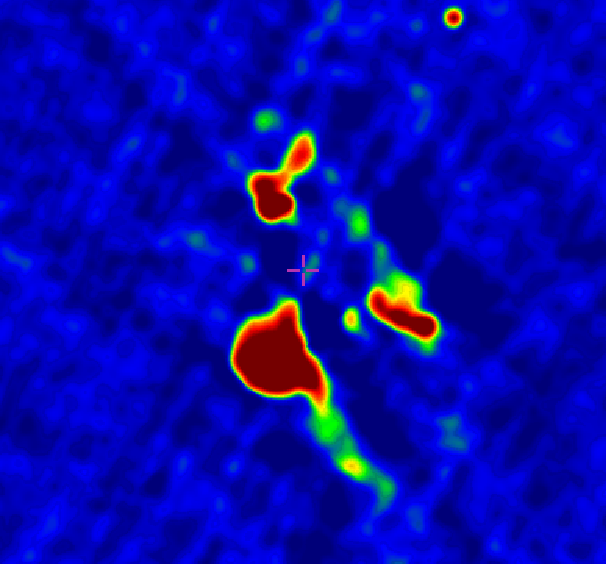
\includegraphics[width=0.48\textwidth]{pics/3c40t-cropped.pdf} \;\;
    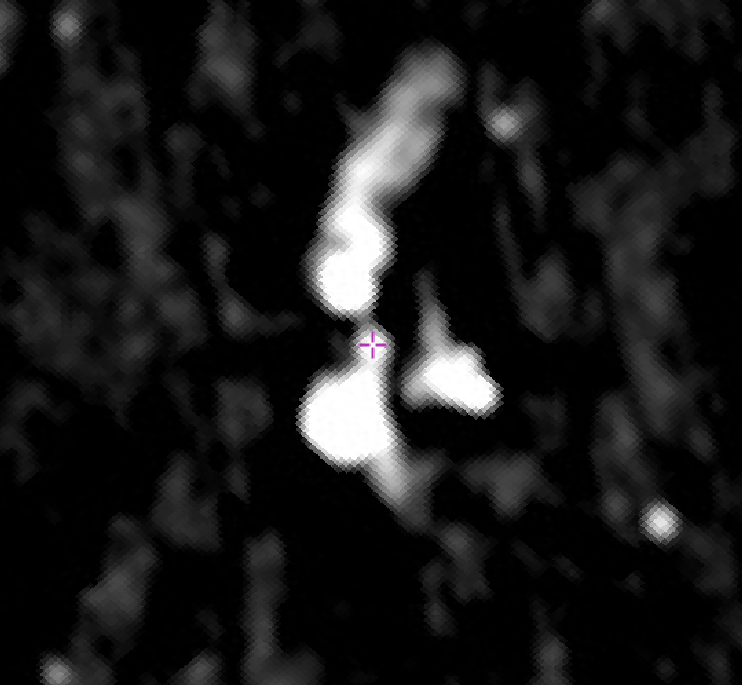
\includegraphics[width=0.48\textwidth]{pics/3c40n-cropped.pdf}
    \caption{Cut-outs centred on 3c40, from TGSS, left; and from NVSS, right. Field of view approximately $\ang{;20;}$ in each: although TGSS has been cropped tighter. Note the absence/presence of the central source (blob).}
    \label{fig:3c40}
\end{figure}

Cross-identification is the non-trivial problem of determining what blobs in one survey come from the same physical objects as those in the other survey. For example, see figure~\ref{fig:3c40} which shows cut-outs from both surveys of the particularly difficult object 3c40 over a field of view of $\ang{;20;}$. The central blob is missing in the lower frequency TGSS but appears in NVSS. In other cases, one large blob in NVSS is split into two smaller blobs in the higher resolution TGSS.
And although 3c40 is comparatively large to the many compact arcsecond sources, there exist degree sized objects up to the extreme radio galaxy Centaurus A, which covers about $\ang{8}$ on the sky (to the Moon's $\ang{0.5}$).\\

There's not one scale that objects exist on, and so there's not one size threshold that'll catch everything that's physical and nothing else. We're looking for physical objects, and cross-identification is what we want to do, but we should expect this to be a hard problem.

\newpage
\subsection{Source catalogues}
\label{sec:source_catalogues}
% explain each of TGSS and NVSS
TGSS catalogues the entire radio sky north of $-\ang{53}$ DEC in 0.6 million sources at 147.5 MHz with resolution $\ang{;;25}$. From TGSS we extract for each source: the source name in IAU form TGSSADR JHHMMSS.S+DDMMSS, the RA and DEC position on the sky (in degrees), the lengths of the major and minor axes of the fitted gaussian (in arcseconds), the integrated (total) flux density (in milli-janskys: mJy) and peak flux (in mJy/beam), and the position angle (orientation on the sky) of the major axis (in degrees).\\

NVSS catalogues the entire radio sky north of $-\ang{40}$ DEC in 2 million sources at 1.4 GHz with resolution $\ang{;;45}$. From NVSS we extract for each source: the source name in IAU form NVSS JHHMMSS+DDMMSS, the RA and DEC position on the sky (in degrees), the lengths of the major and minor axes (in arcseconds), the peak flux (in mJy/beam, uncorrected), the position angle (in degrees), as well as the integrated and peak residual flux (in mJy and mJy/beam), and the integrated polarised flux density (in mJy) with its Stokes Q and U linear polarisation brightnesses (in mJy) measured at the source's centre.

\newpage
\section{Positional matching}
\label{sec:positional_matching}
To do cross-identification, we need a dataset of pairs of sources between the two surveys to then decide whether they match. To this end, we create a common catalogue of pairs of TGSS sources and NVSS sources. However, given roughly a million objects in each survey there's a total of $10^{12}$ possible pairs, so we need an initial filter to reduce the size of the problem, computationally.\\

Positional matching is determining matches purely based on the relative positions (RA and DEC) of each source on the sky. Assuming isotropy, this amounts to only considering the angular separation between their centres (which we calculate using their geodesic distance on the celestial sphere). For compact sources (tight blobs, that subtend a small angle) this is a great filter as we'd scarcely expect two compact blobs on the sky degrees apart to have come from the same physical object. \\

However, in radio, this is not a universal assumption as we have sources, like the aforementioned Centaurus A and 3c40, that cover degrees or many arcminutes on the sky. We take $\ang{;2;}$ as our separation limit when creating pairs from the entire sky. Note that the average number of matches grows as the square of this limit as the area of the disk of possible matches grows. We reject all pairs beyond this limit, so we're at least missing direct matches for the degree sized objects on the sky. With the problem reduced, the elements of our dataset are now positional matches of TGSS sources to NVSS sources within $\ang{;2;}$ instead of general pairs of sources.

\subsection{Positional matching results}
\label{sec:posmatch}
% explain plots and comparison

We initially consider matches of TGSS sources to NVSS sources over the entire sky that both surveys cover (north of $-\ang{40}$ DEC). In part, because we have a reference to the same being done recently in \citet{posmatchpaper}, albeit with some differences. \citet{posmatchpaper} uses a finer separation limit of $\ang{;;30}$ and drops all non-unique matches. When we train a logistic regression classifier in section~\ref{sec:logistic_regression}, we do so on a $\ang{20}\times\ang{20}$ patch of sky but with a separation limit of $\ang{;10;}$, as to reduce the size of the problem further.

% hist_angle
\begin{figure}[H]
    \centering
    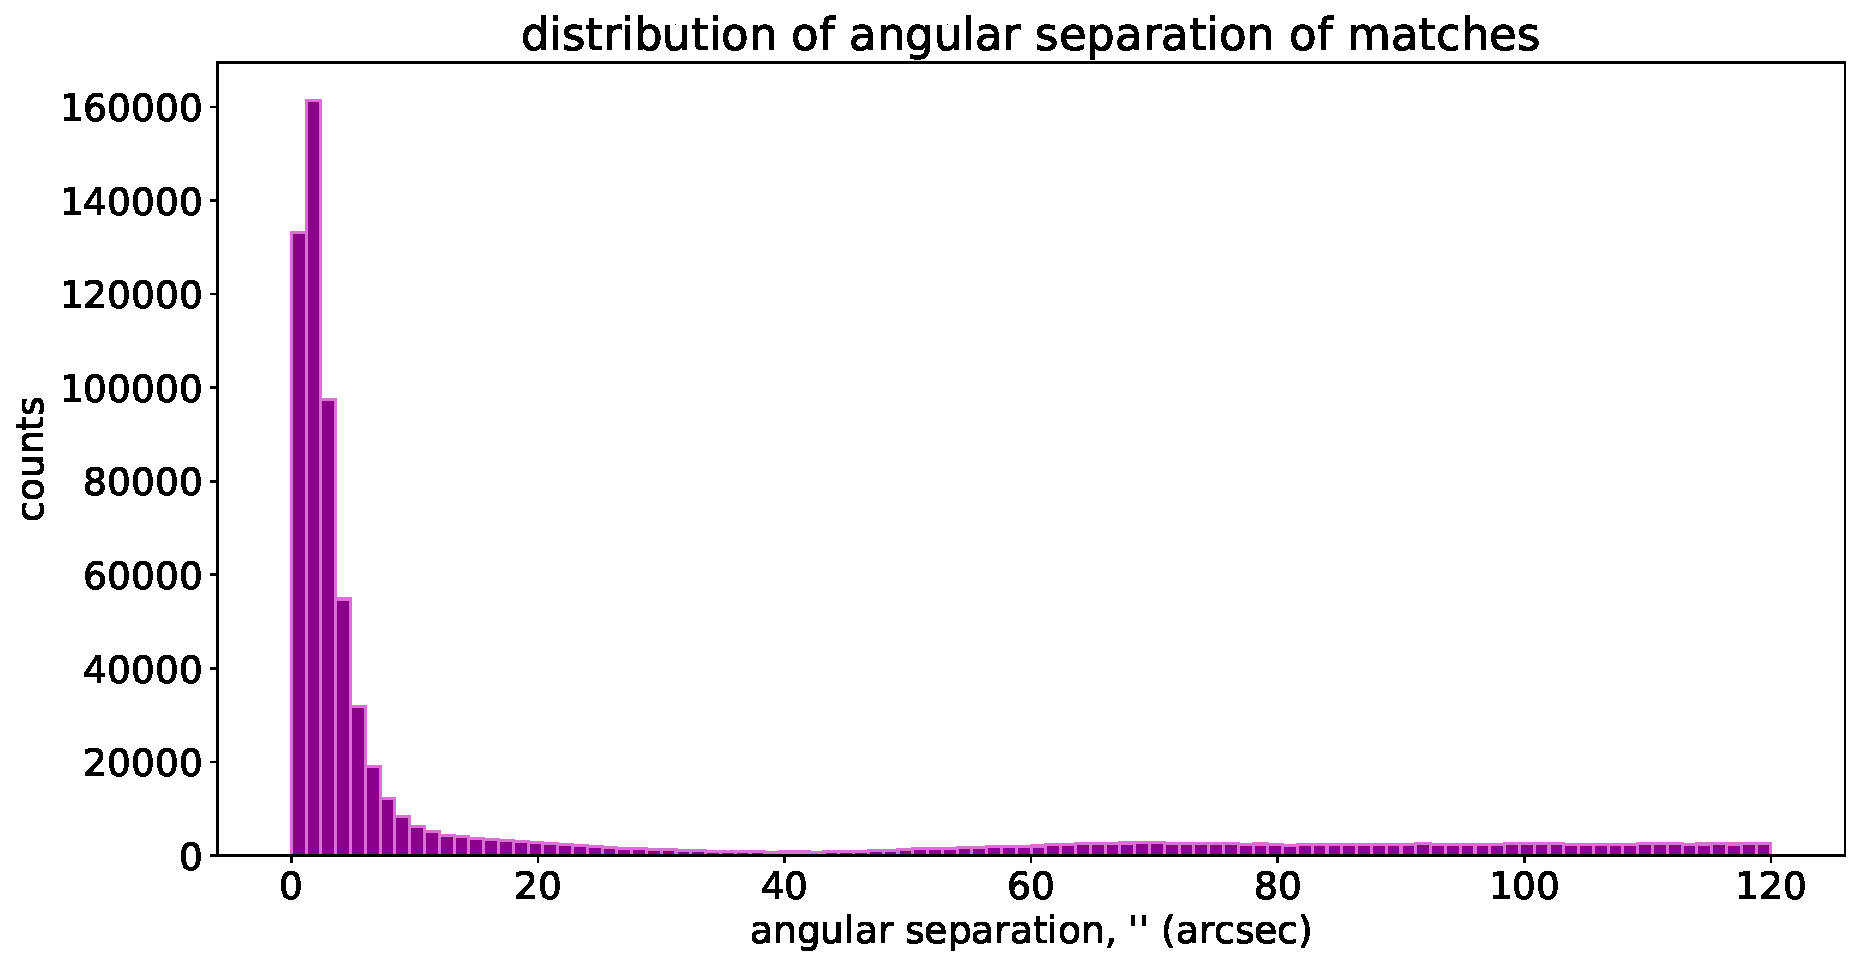
\includegraphics[width=\textwidth]{pics/hist_angle.pdf}
    \caption{Distribution of angular separation of positional matches TGSS-NVSS over entire common sky (north of $-\ang{40}$ DEC) within separation limit of $\ang{;2;}$. Note the bi-modality within this range into two populations either side of $\ang{;;40}$.}
    \label{fig:hist_angle}
\end{figure}

See figure~\ref{fig:hist_angle} for the distribution of separations for matches (TGSS-NVSS) over the entire common sky. In total, we find over 720000 matches within $\ang{;2;}$ in a bi-modal distribution split either side of $\ang{;;40}$ separation, with the vast majority of matches within $\ang{;;10}$ (\citet{tgss} estimates 94.4\% of TGSS sources have a NVSS counterpart within $\ang{;;45}$). To clarify, there are two separate angular distance limits: the match radius $\ang{;2;}$ for getting in the catalogue to be considered at all, and the smaller $\ang{;;40}$ which we observe as a divide between two separate populations.\\

We hypothesise that this bi-modality is the result of two geometric effects: the actual matches between objects and then the start of a long quadratic as the radius of the search window increases and the circle's area collects more and more false matches. It's worth pointing out that we don't see this quadratic increase yet, but would expect it to pick up further out. That is, as we extend the search radius out to $\ang{180}$ we'd expect the curve to be quadratic, until we matched the entire sky. Later, in section~\ref{sec:logistic_regression}, this smaller limit of $\ang{;;40}$ is what we'll use to label positional matches as being `real' or not. To be clear though, we do not actually believe that all the matches within $\ang{;;40}$ are from actual objects.

\subsection{Spectral index}
\label{sec:spectral_index}
We can also look at the distribution of the spectral index, $\alpha$, of the positional matches. The observed spectral index for a TGSS-NVSS match assumes the peak flux follows a power law of frequency, takes the ratio of sources, and re-arranges for the best guess at the exponent ($\alpha$) were the two sources the same object:
\begin{equation}
\label{eq:alpha}
\begin{split}
S_\nu &= \nu^\alpha \\
S_\mathrm{TGSS}/S_\mathrm{NVSS} &= (\nu_\mathrm{TGSS}/\nu_\mathrm{NVSS})^{\alpha_\mathrm{obs}} \\
\alpha_\mathrm{obs} &= \frac{\log(S_\mathrm{TGSS}/S_\mathrm{NVSS})}{\log(\nu_\mathrm{TGSS}/\nu_\mathrm{NVSS})}
\end{split}
\end{equation}
See figure~\ref{fig:hist_alpha_comparison} for the distribution of the observed spectral index of matches over the entire common sky, and a comparison of the same plot from \citet{posmatchpaper}. Note here a mistake (on my part) in that peak flux did not get corrected for beam size for either survey when calculating each match's spectral index. The main distribution appears roughly identical between plots, except for the fatter tails in ours with a right tail preference for higher peak fluxes.\\

Unlike \citet{posmatchpaper}, we did not drop non-unique matches and had a larger separation limit and those must therefore allow matches with more diverse alpha values. This makes sense: the more non-unique matches we allow, the more different we'd expect the sources to be and so the more diverse alpha values we'd allow. These non-unique matches are more likely to false, and so these extreme alpha values are likely unphysical.
% As a note, at one point uniqueness of a match was boolean feature in the catalogue, perhaps this could have been explored further.
We observe that the right tail of false matches preferences higher peak fluxes from TGSS. This follows from a larger TGSS flux giving larger ratio to a fixed NVSS frequency, and so giving a larger $\alpha$ value from the spectral index formula, see equation~\ref{eq:alpha}.\\

% hist_alpha
\begin{figure}[H]
    \centering
    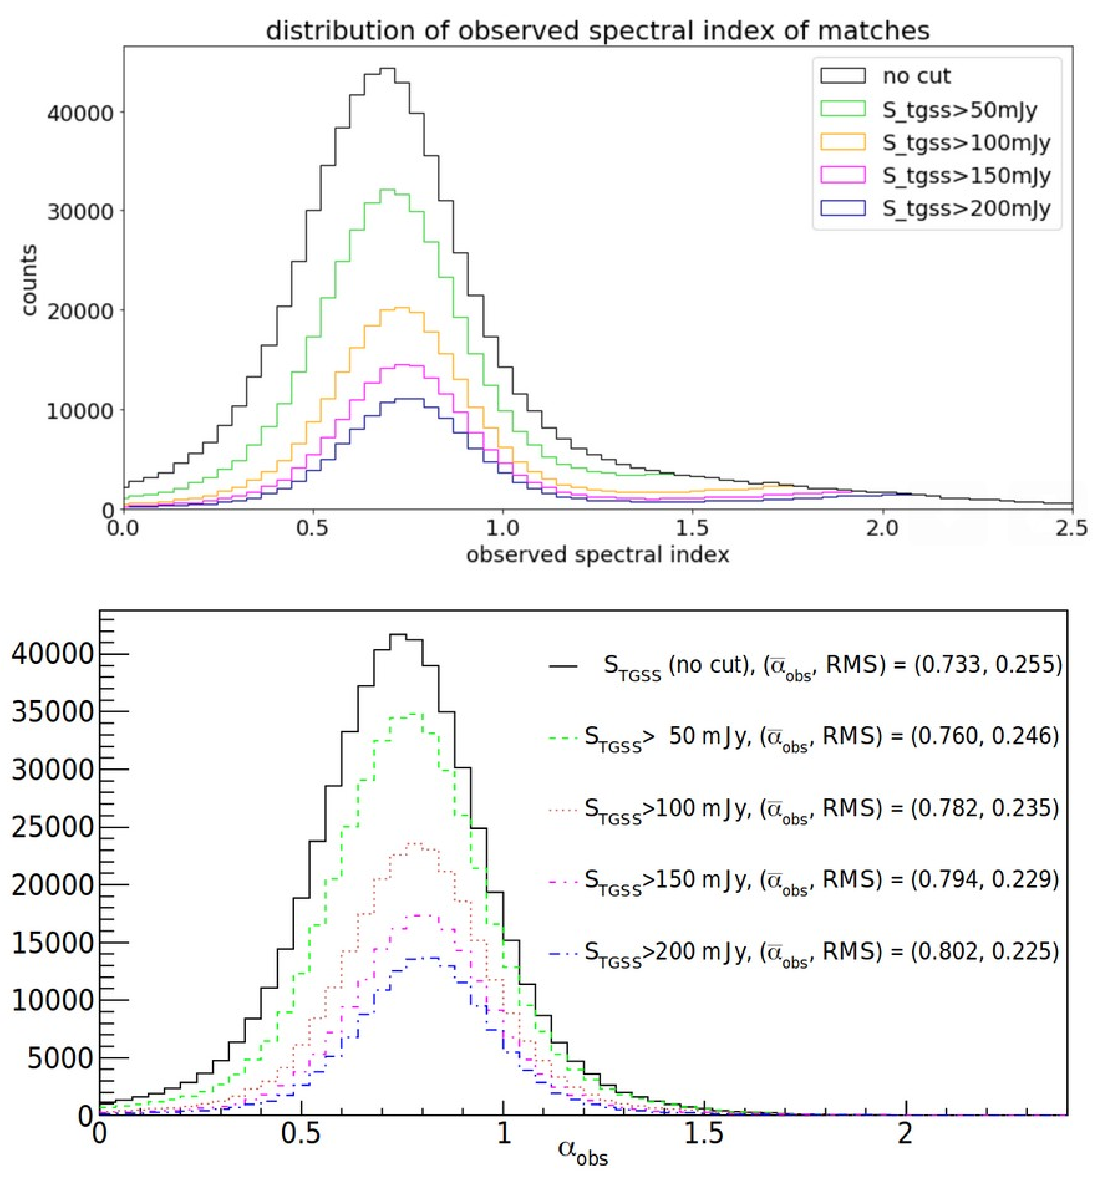
\includegraphics[width=\textwidth]{pics/hist_alpha_comparison-cropped.pdf}
    \caption{Distribution of the spectral index of positional matches over the common sky with cuts at various TGSS peak fluxes overlayed, top; with comparison to the same plot from \citet{posmatchpaper}, bottom (figure used without permission). Note in our distribution the fatter tails and the right tail's preference for higher flux cuts.}
    \label{fig:hist_alpha_comparison}
\end{figure}

\newpage
\subsection{Catalogue of matches}
\label{sec:catalogue_of_matches}
% pair T / N and making the catalogue
% Note: an exact definition of feature vectors and labels will follow in section~\ref{sec:napkin_intro_to_ml}, here we just consider them vaguely.
We construct a common catalogue of the positional matches of TGSS to NVSS over a $\ang{20}\times\ang{20}$ square patch of sky between $(-\ang{35}\mathrm{RA}, \ang{149}\mathrm{DEC})$ and $(-\ang{15}\mathrm{RA}, \ang{169}\mathrm{DEC})$ (i.e.\ centred on $(-\ang{25}\mathrm{RA}, \ang{159}\mathrm{DEC})$), with a separation limit of $\ang{;10;}$. The choice of patch is arbitrary, testing shows no difference if the patch is moved (as long as it stays totally within the common sky), $(\ang{35}\mathrm{S}, \ang{149}\mathrm{E})$ happens to be Canberra's latitude and longitude.\\

The main advantage of making a common catalogue is that we can add derived features from a combination of both sources. See section~\ref{sec:source_catalogues} for details of each of the raw and fitted features from the source catalogues that we save into the common catalogue.\\

The first of the derived features we add is separation. Later, we'll assume isotropy and remove the RA and DEC position values. This is actually an error, as in particular the positional angle, the orientation on the sky of the gaussian fit, no longer gives alignment information about the match. If we insist on dropping the position, then the relative angle of each major axis against the line segment joining the centres should have been used instead.
The disadvantage of making this common catalogue from positional matching is precisely that we must choose some separation limit and rule out degree sized objects, or create a catalogue filled with false matches between unrelated compact sources too far away from each other.\\

The second derived feature that we add is the spectral index. From section~\ref{sec:spectral_index}, we know that the spectral index comes from observing the object at two different frequencies. We also know that most matches fall between 0.5 and 1, and moreover, that extreme spectral indices indicate unphysical matches.\\

The last derived features are the logarithm of the various flux features from section~\ref{sec:source_catalogues}, and the logarithm of the peak flux ratio (as in the spectral index equation~\ref{eq:alpha}). Taking the logarithm is a common technique for treating the large scale that fluxes can fall over. Note that these logarithm features weren't saved into the created catalogue.
% The disadvantage to this approach is that we impose positional matching onto the dataset three times over: we only allow sources within a $\ang{20}$ patch, only allow matches within $\ang{;10;}$, and we label 1 any matches within $\ang{;;40}$. However, despite examples like Centaurus A, we argue that this can be treated as positional matching for compact sources, and that the loss of degree sized objects is worth it computationally.
% Note that unlike the other two derived features (separation and spectral index) this doesn't combine catalogues.

\newpage
\section{Logistic regression}
\label{sec:logistic_regression}
Having created a dataset, and along the way recreated existing positional matching results, we now return to the central problem of cross-identification to find physical objects. Due to the large number of matches in the catalogue, we want to train an automated classifier to perform this task. With our common catalogue of TGSS to NVSS positional matches, we choose to approach this problem as a binary classification task. Given a positional match between a TGSS source and a NVSS source, tell whether the sources come from the same physical object.\\

It's worth noting that binary classification, let alone this variation, is not the only way to approach cross-identification. We could instead aim to train a predictor to take any TGSS source and return the best match in NVSS, or take a list of sources and return the likelihood of them all coming from the same object, or take a position on the sky (RA, DEC) and return the nearest object, etc. We choose binary classification on a TGSS-NVSS pair of sources, for its simplicity and how can input directly from the positional matching catalogue we've made.

\subsection{A napkin-sized introduction to machine learning}
\label{sec:napkin_intro_to_ml}
Supervised machine learning consists of a function, $f: X \rightarrow Y$
\begin{itemize}
    \item[$f$] is the function: called the classifier/predictor, of some form (called the model)
    \item[$X$] is the input: real-valued vectors from some space $\mathbb{R}^D$, where each component is called a feature and the inputs are called feature vectors
    \item[$Y$] is the output: predictions of some type, to be compared against labels (of a similar type). Note that a later decision on the predictions may need to be made to compare directly.
    % predictions/labels are not necessarily real-valued scalars and decisions may need to be forced to transform predictions to the form of the labels
\end{itemize}
We consider how this function acts on data: known inputs and their corresponding labels, i.e.\ a dataset $\{(\vec{x_1},\hat{y_1}), \ldots, (\vec{x_N},\hat{y_N})\}$.
% Where a distinction between the initial form of the predictions and form of the labels.
Here, $\hat{y_i}$ is the known label associated with a feature vector $\vec{x_i}$, and $y_i = f(\vec{x_i})$ the prediction that the function makes for that input. While $\hat{y_i}$ and $y_i$ may not be exactly the same type (e.g.\ $\{0,1\}$ and $[0,1]$), we assume some decision exists for the prediction to be directly comparable to the label (e.g.\ $y_i \geq 0.5$).%\\

\newpage
Three related algorithms, all separately called `machine learning', concern this function, $f$:
\begin{itemize}
    \item[(1)] training: optimising the function against training data
    \item[(2)] testing/prediction: evaluating the function on other, testing data
    \item[(3)] hyperparameter tuning/model selection: changing the other (non-input) arguments or the model (i.e.\ the form) of the function, as well as changing the training (e.g.\ changing the regulariser $\lambda$: the penalty to over-fitted, complex models)
\end{itemize}

Training is optimising some objective for the function. With labels, this objective is often to minimise a cost function. We consider cost functions of the form: the average of some loss function over the training data plus a regularisation term (with hyperparameter $\lambda$). Loss functions are a metric of the gap between a prediction and a label, i.e.\ $\text{loss}_i = l(\hat{y_i},f(\vec{x_i}))$ (see section~\ref{sec:loss} for more on loss). An example cost function would be $\text{avg loss} + \lambda\,\norm{\vec{\theta}\,}^2$, which would penalise models that weighted many features. These three terms are very similar but operate on different scales: loss is at a particular data point, cost is over the whole training dataset, and the objective is the generalised goal of the training process.\\

Logistic regression is when the model (i.e.\ the form of the function) is:
\begin{equation}
\begin{split}
    f(\vec{x}\,) &= \sigma(\vec{\theta}\cdot\vec{x}+\theta_0) \\
    \sigma(x) &= \frac{1}{1+e^{-x}}       
\end{split}
\end{equation}
Where $\sigma$ is the logistic sigmoid, $\vec{\theta}$ the weights, and $\theta_0$ the bias. Compared to linear regression with $g(\vec{x}\,) = \vec{\theta}\cdot\vec{x}+\theta_0$. One can think that the whole function is really $f(x;\vec{\theta},\theta_0)$ and that training is adjusting these weight/bias arguments. Because logistic regression evaluates a linear combination of all the features at once, it is part of the model class of linear classifiers.

\subsection{Feature vectors and labels}
In the language of the previous section, we set up a logistic regression binary classifier to take in feature vectors (pairs) from the common patch catalogue and return the prediction of the likelihood of the match being real.\\
% Remembering that the catalogue is of a $\ang{20}$ patch with separation limit $\ang{;10;}$, rather than the entire shared sky.\\

Formally, translating raw data (z), in whatever form, through a feature map ($\phi$) into real-valued feature vectors ($\vec{x}$\,) is the work of a `domain expert' (we'll use these symbols in equation~\ref{eq:predictionprocess}). In our case, all of the data in the common catalogue is already numerical (except the source names). For our feature map, we drop the RA and DEC positions and add in logarithm values of the flux and flux densities but otherwise don't alter the catalogue. Another domain expert could add far more complicated features. In a sense, the real domain expertise came much earlier in the construction of TGSS and NVSS from truly raw photometric/geometric data.\\

Finding labels and justifying them is the main obstacle to supervised machine learning. By the arguments in section~\ref{sec:posmatch}, in particular the observation of the distinct population of separations less than $\ang{;;40}$ in figure~\ref{fig:hist_angle}. We choose to use positional matching to label all matches with separation less than $\ang{;;40}$ as a positive match, and all those with separation greater than $\ang{;;40}$ as a negative match. For those within the threshold of $\ang{;;40}$, we create a linear separation score that is 0 at $\ang{;;40}$ and is 1 at a separation of zero. On a technicality, we end up actually placing the threshold at $\ang{;;36}$, this should have been at $\ang{;;40}$.
See figure~\ref{fig:patch_scores_dist} for a plot of these scores over the patch. And see appendix~\ref{app:scorers} for a note on other explicit scorers made. Note that logistic regression generally assumes that all the features have been normalised, which our haven't; and binary classification generally assumes that the labelled population sizes are roughly equal, which ours are (at 63\% negative(0) to 37\% positive(1)).
% patch_scores_dist
\begin{figure}[H]
    \centering
    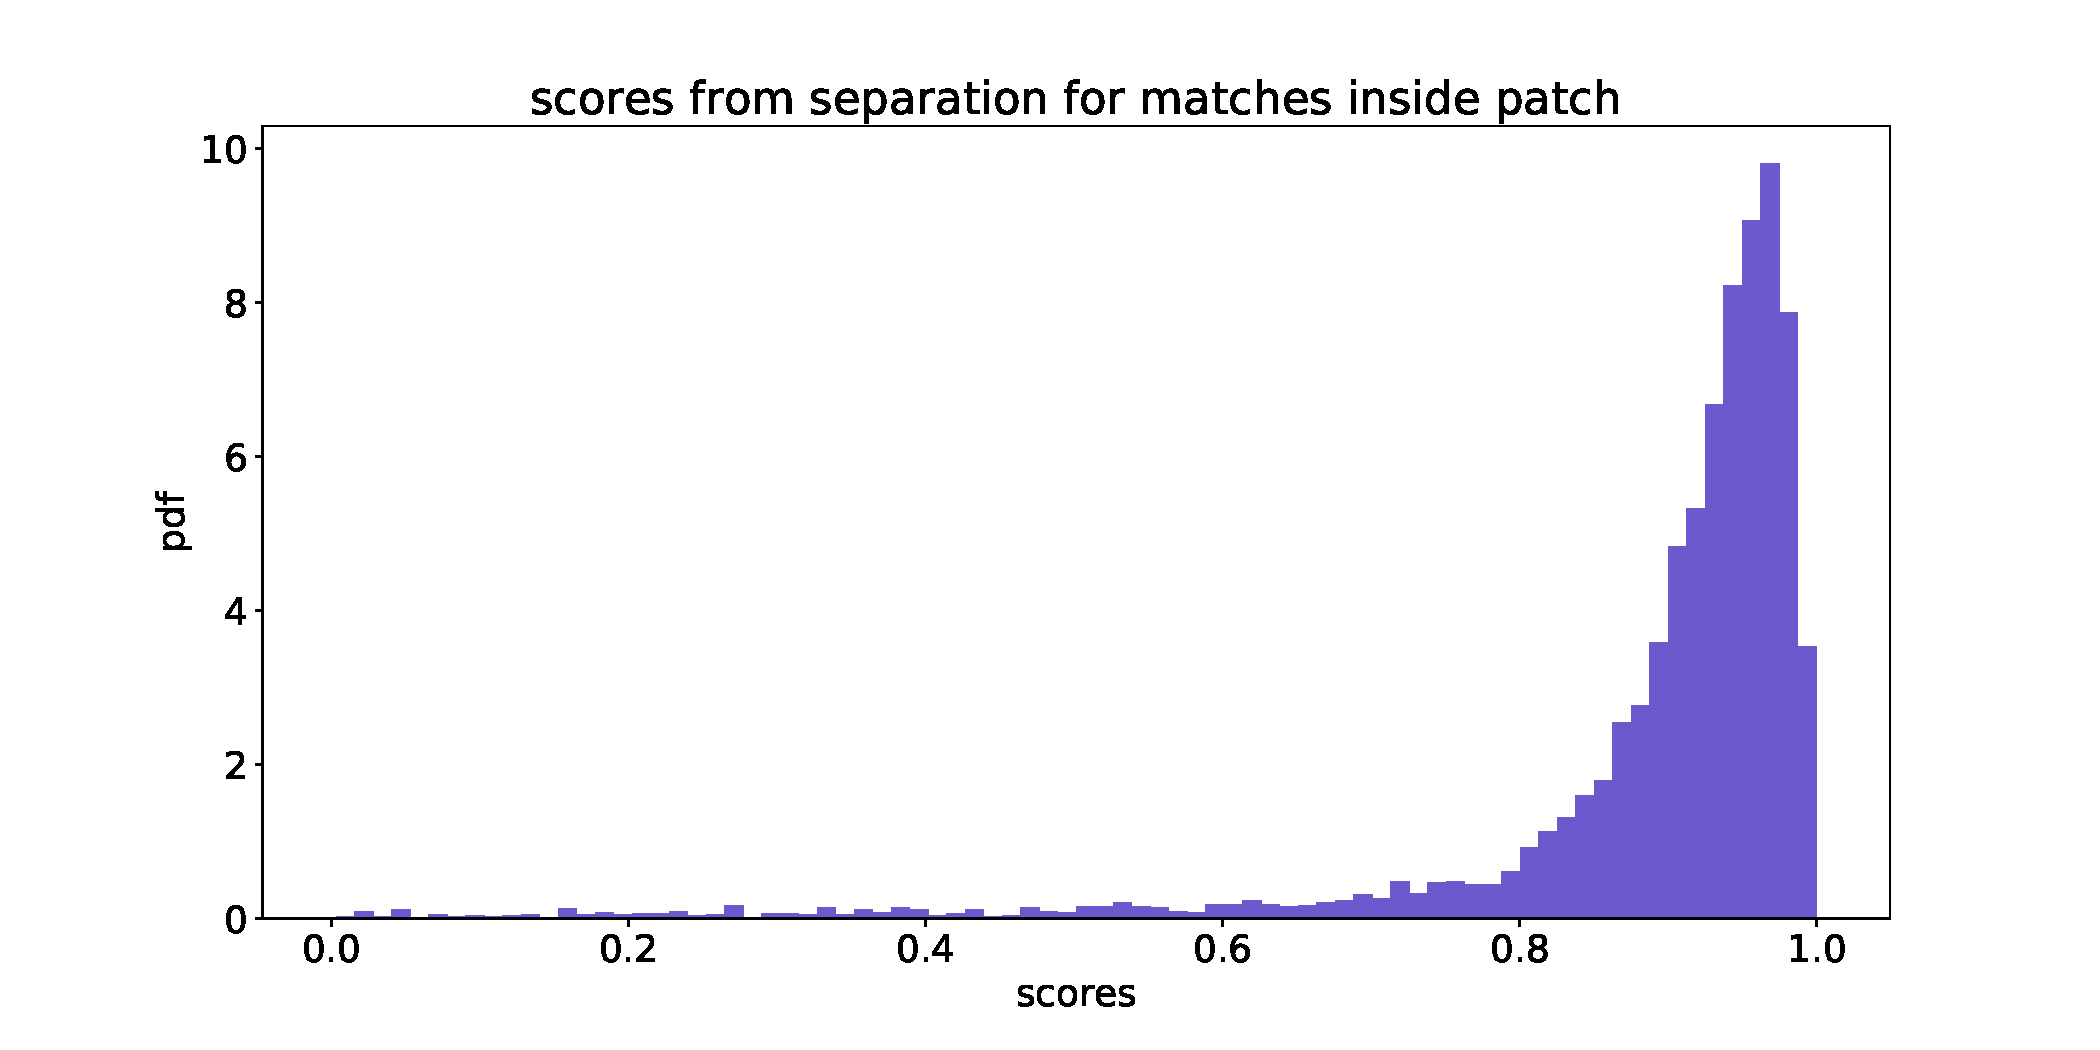
\includegraphics[width=\textwidth]{pics/patch_scores_dist.pdf}
    \caption{Normalised distribution (pdf: probability density function) of linear separation score with threshold at $\ang{;;40}$, for all matches in patch.}
    \label{fig:patch_scores_dist}
\end{figure}

\newpage
\subsection{Loss}
\label{sec:loss}
%  |      | l
%  | 1    | __
We use the binary cross-entropy (BCE) of labels against predictions as our loss term. Information theoretically, this represents the average information gain ($-\log_2{\mathrm{(prob)}}$) over the labels from observing the correct prediction, or the average coding length (in bits) of the labels given lengths optimised for the predictions. This is closely related to the Kullback-Leibler Divergence between the label and prediction distributions, $D_{KL}(\mathrm{labels}\,\rvert\rvert\,\mathrm{predictions})$. Being binary means that the labels can be treated as taking the values $y_n = 0 \mathrm{\;or\;} 1$. Let $f_n$ be the corresponding prediction to a particular label, with n observations going from 1 to the sample size N. Then we have the following derivation of the average loss.
\begin{equation}
\label{eq:BCE}
\begin{split}
    H_f(y) = \mathbb{E}_y [- \log_2(f)] = - \sum_{i} (y_i \log_2(f_i))
    \stackrel{*}{=} - (y \log_2(f) + (1-y) \log_2(1-f)) \\
    \therefore\; \mathrm{average\; loss} = \mathbb{E}_n [{H_f}_n(y_n)] = -\frac{1}{N} \sum_{n=1}^N (y_n \log_2(f_n) + (1-y_n) \log_2(1-f_n))    
\end{split}
\end{equation}
Note the trick in the last equality of the first line (*) of equation~\ref{eq:BCE} that uses the binary label to explicitly write out both cases. Cross entropy can also be notated as $H(y,f)$, but this confuses it with joint entropy. Using this we can derive the average loss, which here equals the cost (which is the objective) as we've set a null regulariser ($\lambda=0$). This form of the average loss is also the negative of the log-likelihood, so minimising this average loss is the same as maximising the likelihood of successfully observing the labels. This is a good motivation to use the binary cross entropy as our loss function.\\

During training, the algorithm is told to minimise the objective (the average loss above) by gradient-descent. Again, here the regulariser is set null so the average loss is the cost, is the objective. In pytorch \citep{torch} this is performed by backpropagation through automatic differentiation. Backpropagation is essentially the chain rule of differentiation except applied along each sub-calculation throughout the function, instead of to the entire function symbolically. This means that evaluating the function and evaluating its derivative have the same complexity since they follow the same set of sub-calculations. Having found the gradient vector, you gradient-descend by taking a tiny step in the opposite direction, then repeat the whole training cycle again.
% (recalling that the gradient vector points at the steepest uphill section and we want to minimise). Given a nowhere constant, differentiable (smooth is better) function over a compact domain this process will reach a local minimum or the boundary. Noting that odd behaviour can happen around a minimum due to the length of the step taken, one may end up oscillating about the minimum.

\newpage
\subsection{Logistic regression results}
% results
It is worth informally remarking here that actually running logistic regression, after feature vectors and labels were all set up, went particularly fast. Leading to the remark: `and I thought machine learning was difficult'! In this lies what I identify as the `TV Chef Problem': if all the ingredients are prepared earlier, the task looks easy. However, this hides that sourcing and preparing those ingredients (mapping data to feature vectors and creating labels), as well as determining if you've even got the right recipe (choosing models and tuning hyper-parameters), to actually serving the meal (interpreting results) is where the real difficulty and ambiguity lies. Watching the TV Chef is effortless, but answering `is this meal right?' can be really hard.\\

We implemented logistic regression in pytorch \citep{torch}, by training a binary classifier on half the feature vectors from the common catalogue against positional matching labels with loss given by the binary cross-entropy. See figure~\ref{fig:torch_lr_weights} for the weights, $\vec{\theta}$, of the model after training. Clearly, the classifier figures out that separation is very important, and places secondary weight on the spectral index and the logarithm of the two peak fluxes.\\

If we remove separation, as it's the feature that we know directly gives the label, we see figure~\ref{fig:torch_lr_weights_nosep} for the weights after training. Now, spectral index and the log peak fluxes dominate. Note that NVSS is preferenced in weight over TGSS. This is likely that TGSS is brighter, a distinction that would have been removed if we'd properly normalised, and could also be due to not correcting for the beam sizes. See appendix~\ref{app:losses} and figure~\ref{fig:torch_lr_losses_nosep} for the loss curve over the training cycles (epochs), it decreases and then appears to stabilise. This is a check to see if training has converged the function to some local solution in the allowed cycles.

\newpage
% torch_lr_weights
\begin{figure}[H]
    \centering
    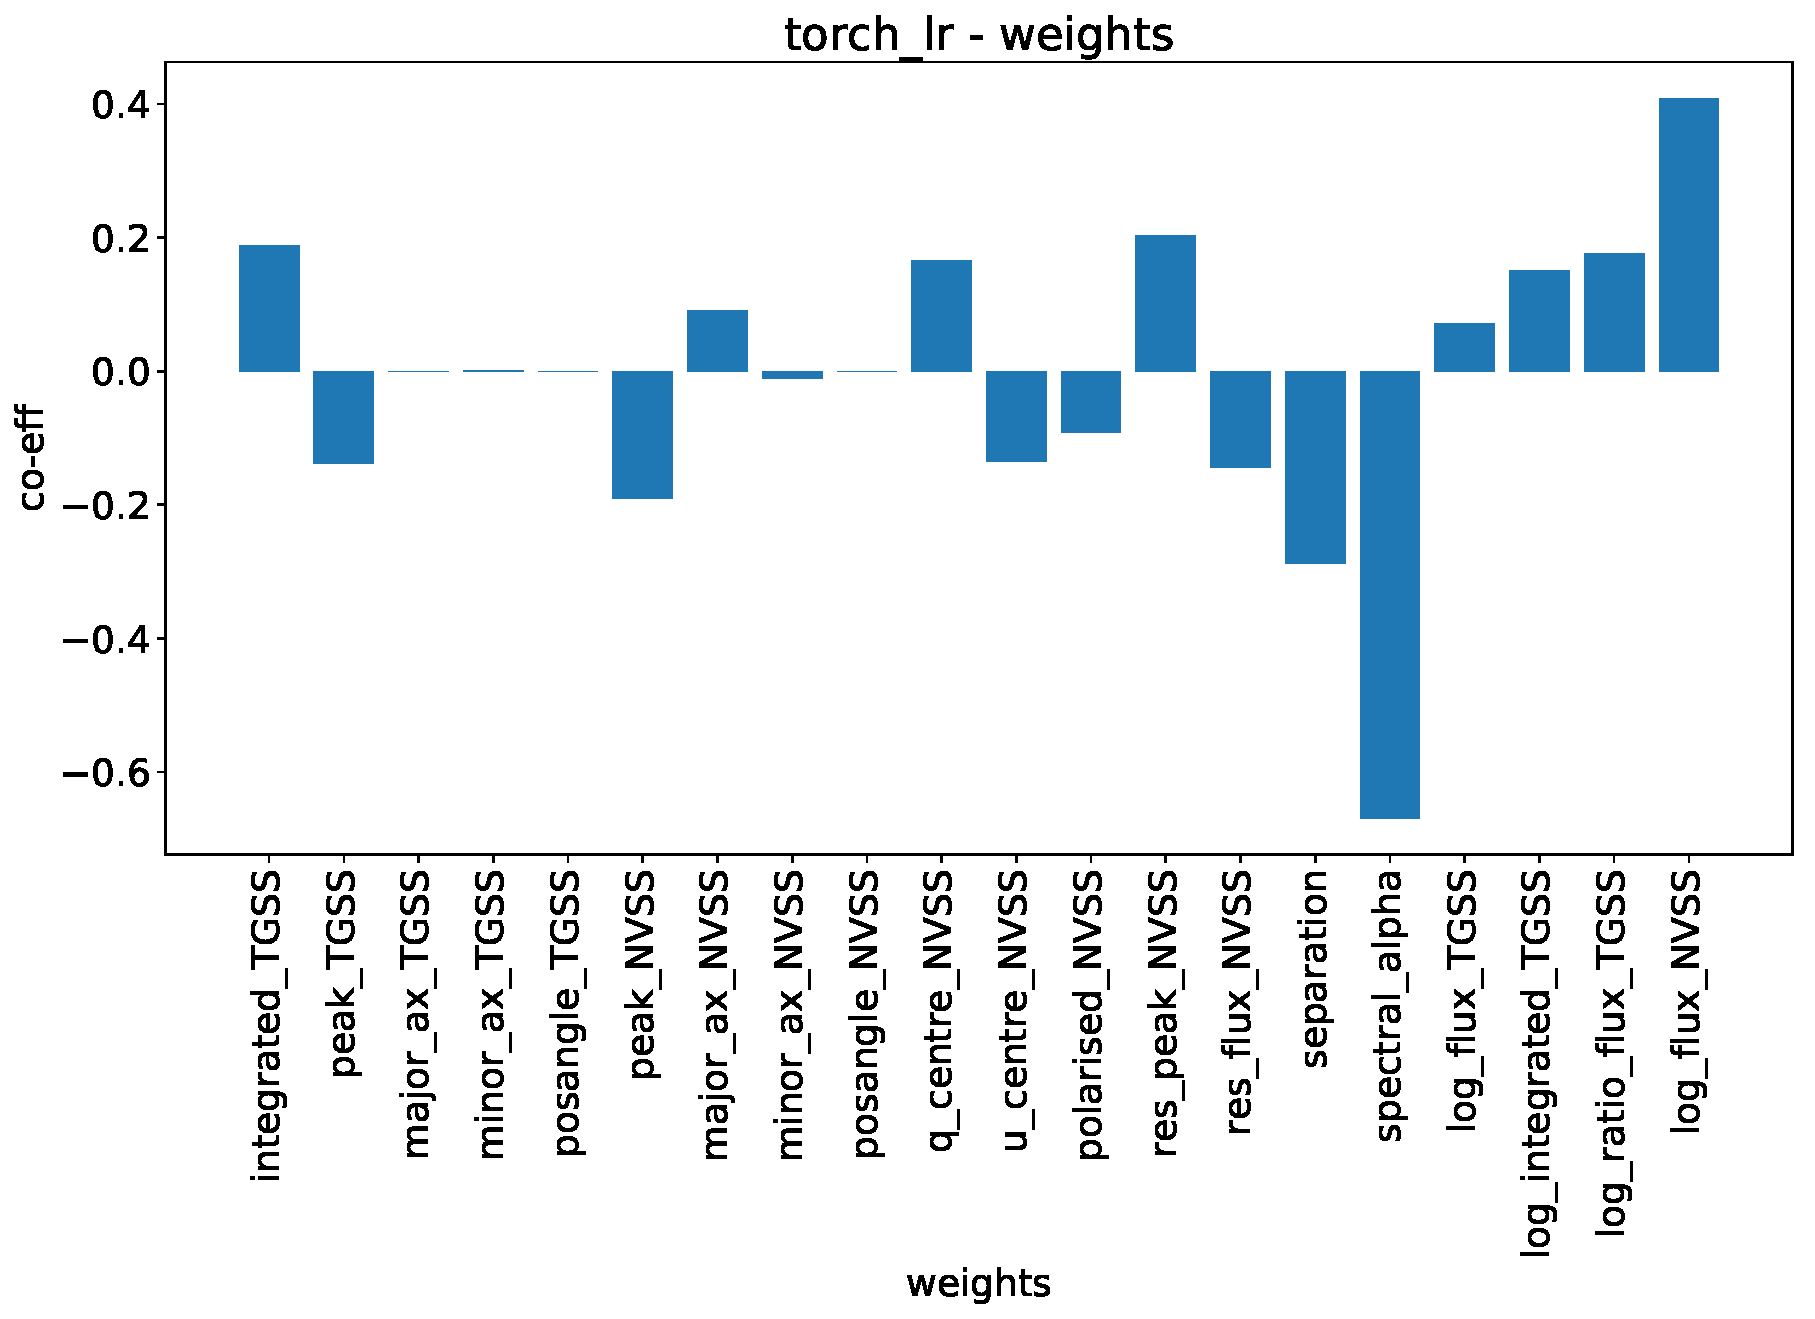
\includegraphics[height=0.41\textheight]{pics/torch_lr_weights.pdf}
    \caption{Weights in pytorch logistic regression model with all features after training, over patch of sky.}
    \label{fig:torch_lr_weights}
\end{figure}

% torch_lr_weights_nosep
\begin{figure}[H]
    \centering
    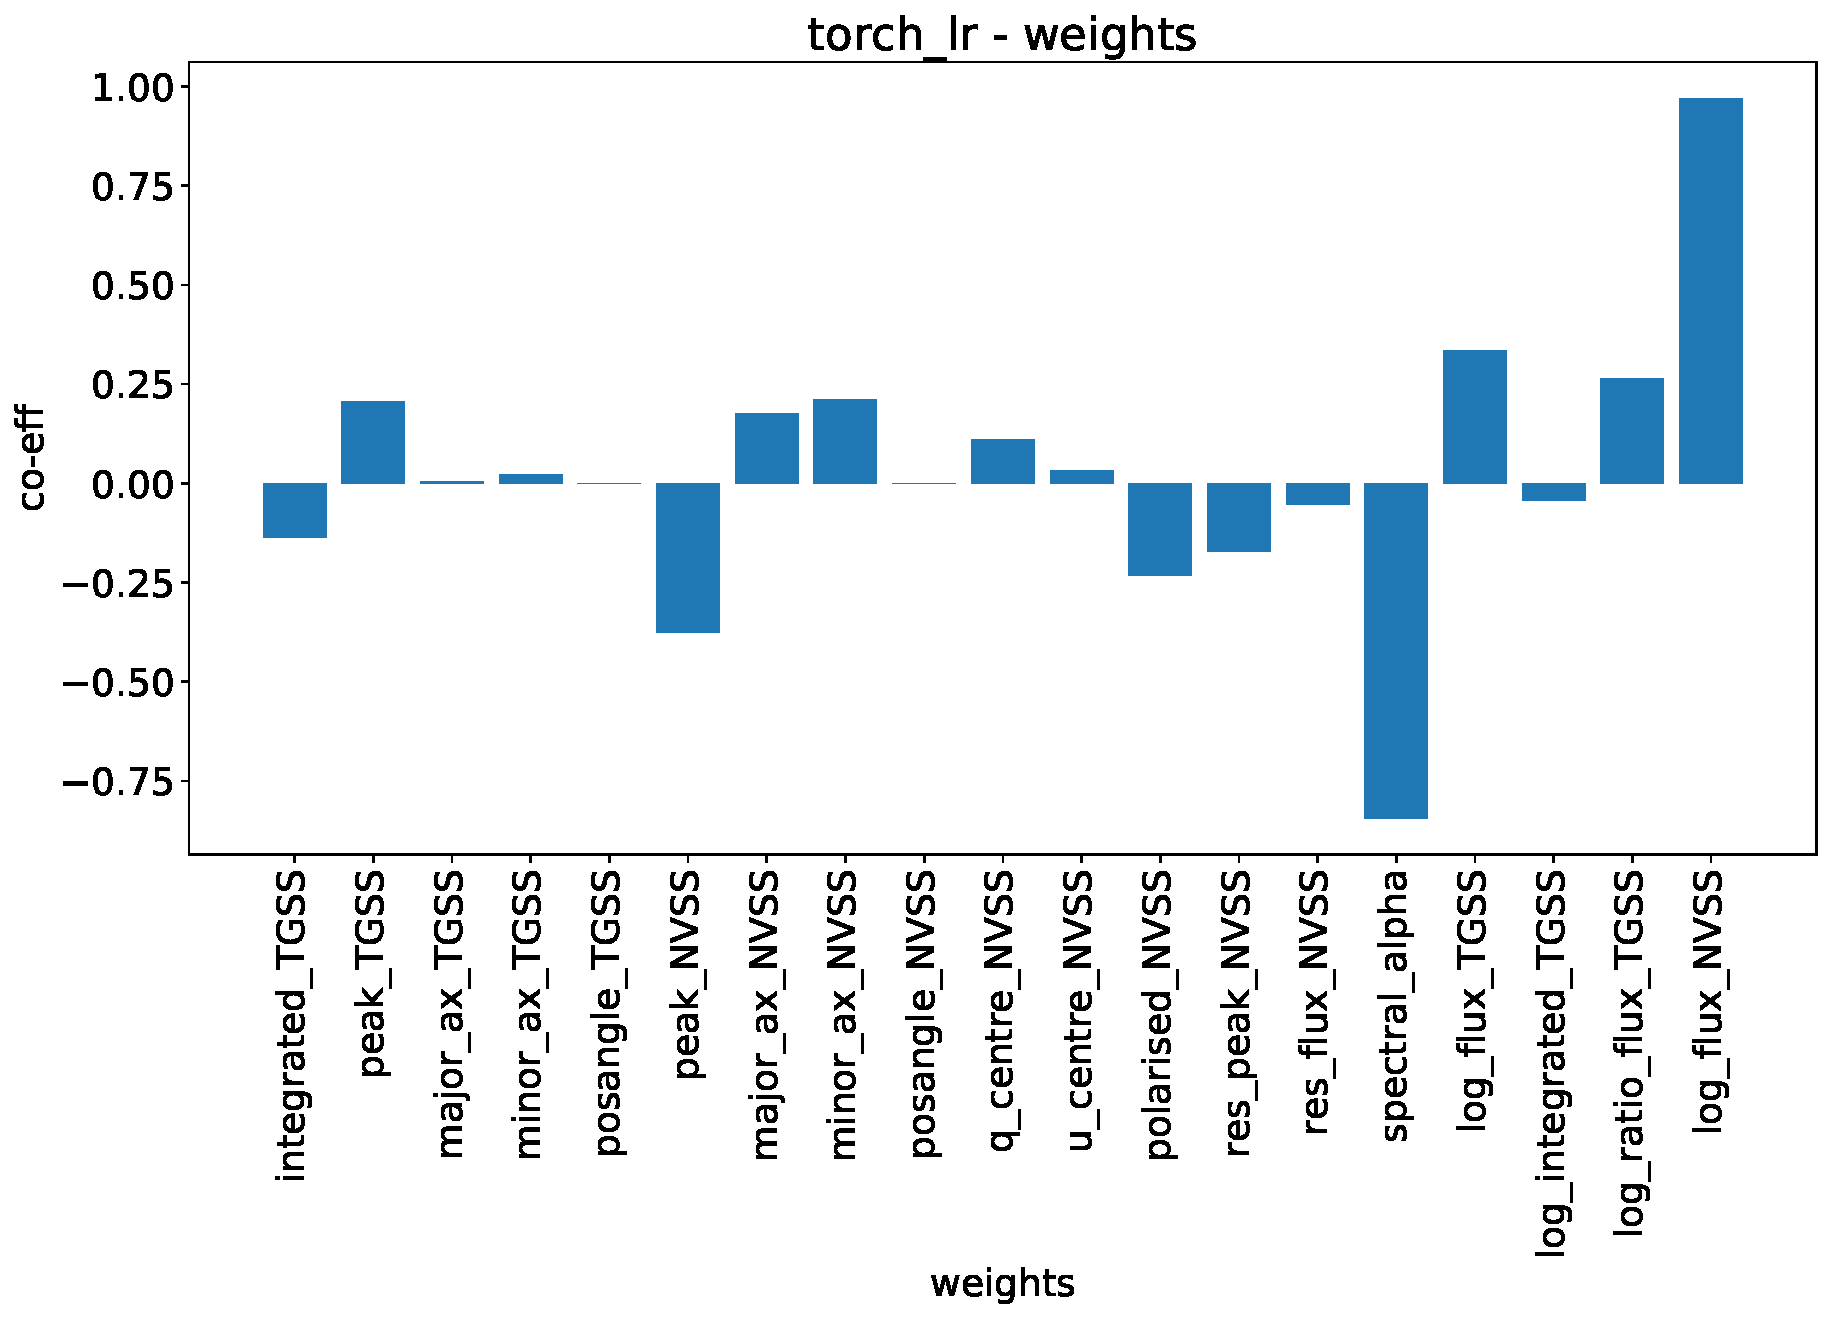
\includegraphics[height=0.41\textheight]{pics/torch_lr_weights_nosep.pdf}
    \caption{Weights in pytorch logistic regression model without separation after training, over patch of sky.}
    \label{fig:torch_lr_weights_nosep}
\end{figure}

% accuracy table
\begin{table}[ht]
\centering
\resizebox{\textwidth}{!}{%
\begin{tabular}{rl|c|c|c}
 &  & \multicolumn{1}{r|}{accuracy} & \multicolumn{1}{r|}{precision} & \multicolumn{1}{r}{recall} \\ \hline
\multirow{2}{*}{\begin{tabular}[c]{@{}r@{}}pytorch:\\ all features\end{tabular}} & over patch catalogue & 75.7 & 42.3 & 90.2 \\ \cline{2-5} 
 & over manual labels & 80.0 & 80.0 & 100 \\ \hline
\multirow{2}{*}{\begin{tabular}[c]{@{}r@{}}pytorch:\\ no separation\end{tabular}} & over patch catalogue & 70.3 & 36.9 & 88.2 \\ \cline{2-5} 
 & over manual labels & 80.0 & 80.0 & 100 \\ \hline
\multirow{2}{*}{scikit-learn} & over patch catalogue & 97.4 & 90.2 & 96.3 \\ \cline{2-5} 
 & over manual labels & 82.5 & 100 & 78.1
\end{tabular}%
}
\caption{Accuracy percentages for logistic regressions against positional matching and manual labels, after training on half the catalogue. Showing pytorch results for the model with all features and for the model with all minus separation, as well as scikit-learn (sklearn) results using all features (see appendix~\ref{app:sklearn} for scikit-learn).}
\label{tab:accuracy}
\end{table}

To quantify the success of these classifiers, see table~\ref{tab:accuracy} for percentages of accuracy (proportion correctly predicted), precision (proportion predicted true that are labelled true), and recall (proportion labelled true that are predicted true), when tested against both the whole catalogue and some manual labels. The manual labels are a set of 40 labels generated by eye (thanks to Matthew Alger for half of them) from directly comparing the cut-outs of TGSS and NVSS. Clearly from the table, they were not a particularly discerning set of objects and the classifiers predicted them easily. This is a reminder that positional matching does sometimes suffice, especially when the same source appears in both surveys. We also performed the same logistic regression in scikit-learn, which proved faster and more accurate, the main difference being that it had regularisation.\\
% Remember though that we know that there are objects like 3c40 and Centaurus A that aren't even in the catalogue to deny, so these accuracies are all conditioned on the feature vectors and labels we're concerning.

% Observing the top four lines of table~\ref{tab:accuracy}, and
Comparing these accuracies to the label proportion of 63\%/37\%, we can conclude that the classifier does manage to predict positional matching to some degree. That recall is heavily preferenced against precision, means that the classifier says a lot of matches are true, including most of the labelled true ones, but a lot more of the false ones.
% The last two lines are for when we checked the pytorch result by running the same logistic regression through scikit-learn (see \ref{app:sklearn}), the main difference being that sklearn had regularisation and so really leaned heavily on separation and recovered far higher accuracies.
That scikit-learn performed so much better than our implementation is a lesson in the importance of regularisation. And in choosing the right type of regulariser: here one that favours using few features was beneficial as we have a single feature (separation) with lots of information about the label, but the same regulariser would do poorly if we had lots of features that each told us a little about the label.\\

\subsection{Predictions}
% explain f, g, and h  and the three types of predictors
% plot prediction histograms with labelled populations, two humps

We've addressed in section~\ref{sec:napkin_intro_to_ml} that generalised predictions can take any form. Here, we'll consider the cases for predictions that are a scalar value. We can continue the process from the raw data (z) through the feature map ($\phi$) into real-valued feature vector ($\vec{x}$\,). From here we apply our model function which we assume outputs some prediction in $\mathbb{R}$, which we call a score. We'll see two other types of scalar predictors here.\\
{\large
\begin{equation}
    \label{eq:predictionprocess}
    z \xrightarrow{\mathmakebox[3em]{\phi}} \bigg\rvert \; \vec{x} \xrightarrow{\mathmakebox[3em]{score}} \mathbb{R} \xrightarrow{\mathmakebox[3em]{\sigma}} [0,1] \xrightarrow{\mathmakebox[3em]{decision}} \{0,1\}
\end{equation}}
Where the vertical line in equation~\ref{eq:predictionprocess} represents the transition of the problem from one in the domain to one in a machine learning framework. To the predicted score we can then apply some bounding function that respects the ordering, like the logistic sigmoid within logistic regression. Without loss of generality, we assume that this bounded function outputs values within $[0,1]$. Suggestively, this lets us read the value off as a class probability, our second type of scalar predictor after score. Finally, we can make a decision on the class probability to directly compare to the boolean labels. Having predictions as boolean classes is the third type of predictor. Note that this decision doesn't have to be around a threshold, but we'll treat it as one here. And that we don't make this decision when calculating loss, where we use the score or probability predictions. \\

The default threshold is 0.5 and would have the classifier composed with a step function predict the negative class for scores in $[0,0.5[$ and the positive class for those in $[0.5,1]$. However, we run into an issue, with imbalanced classes and no regularisation, the classifier ends up predicting nearly all of the matches as negative and just scores the un-conditioned accuracy of 63\% (with terrible recall). Instead, we choose to place the threshold exactly at the divide in the labelled positive and negative classes. This is somewhat artificial, but still serves to evaluate the success of the classifier.\\

See figure~\ref{eq:predictionprocess} and note the non-standard names of $h(x),g(x),f(x)$ for the functions that predict score, probability, and class respectively, and that all the distributions are normalised, so that the 63\%/37\% class bias for the testing data isn't shown. We show the predictions from the pytorch classifier (with all features) but with the two label classes in separate distributions. Clearly, we see a split that represents the accuracies in table~\ref{tab:accuracy}: the classes overlap but show a definite bias either side. The third plot shows the decision using the classifier, with the threshold artificially placed at the crossing point of the classes in the second plot (0.17). Again, we see a fuzzy but definite distinction between the classes.\\

Overall, by appealing to the weights, accuracies, and class predictions, we conclude that logistic regression does successfully predict positional matching labels. 

% torch_lr_predictions
\begin{figure}[H]
    \centering
    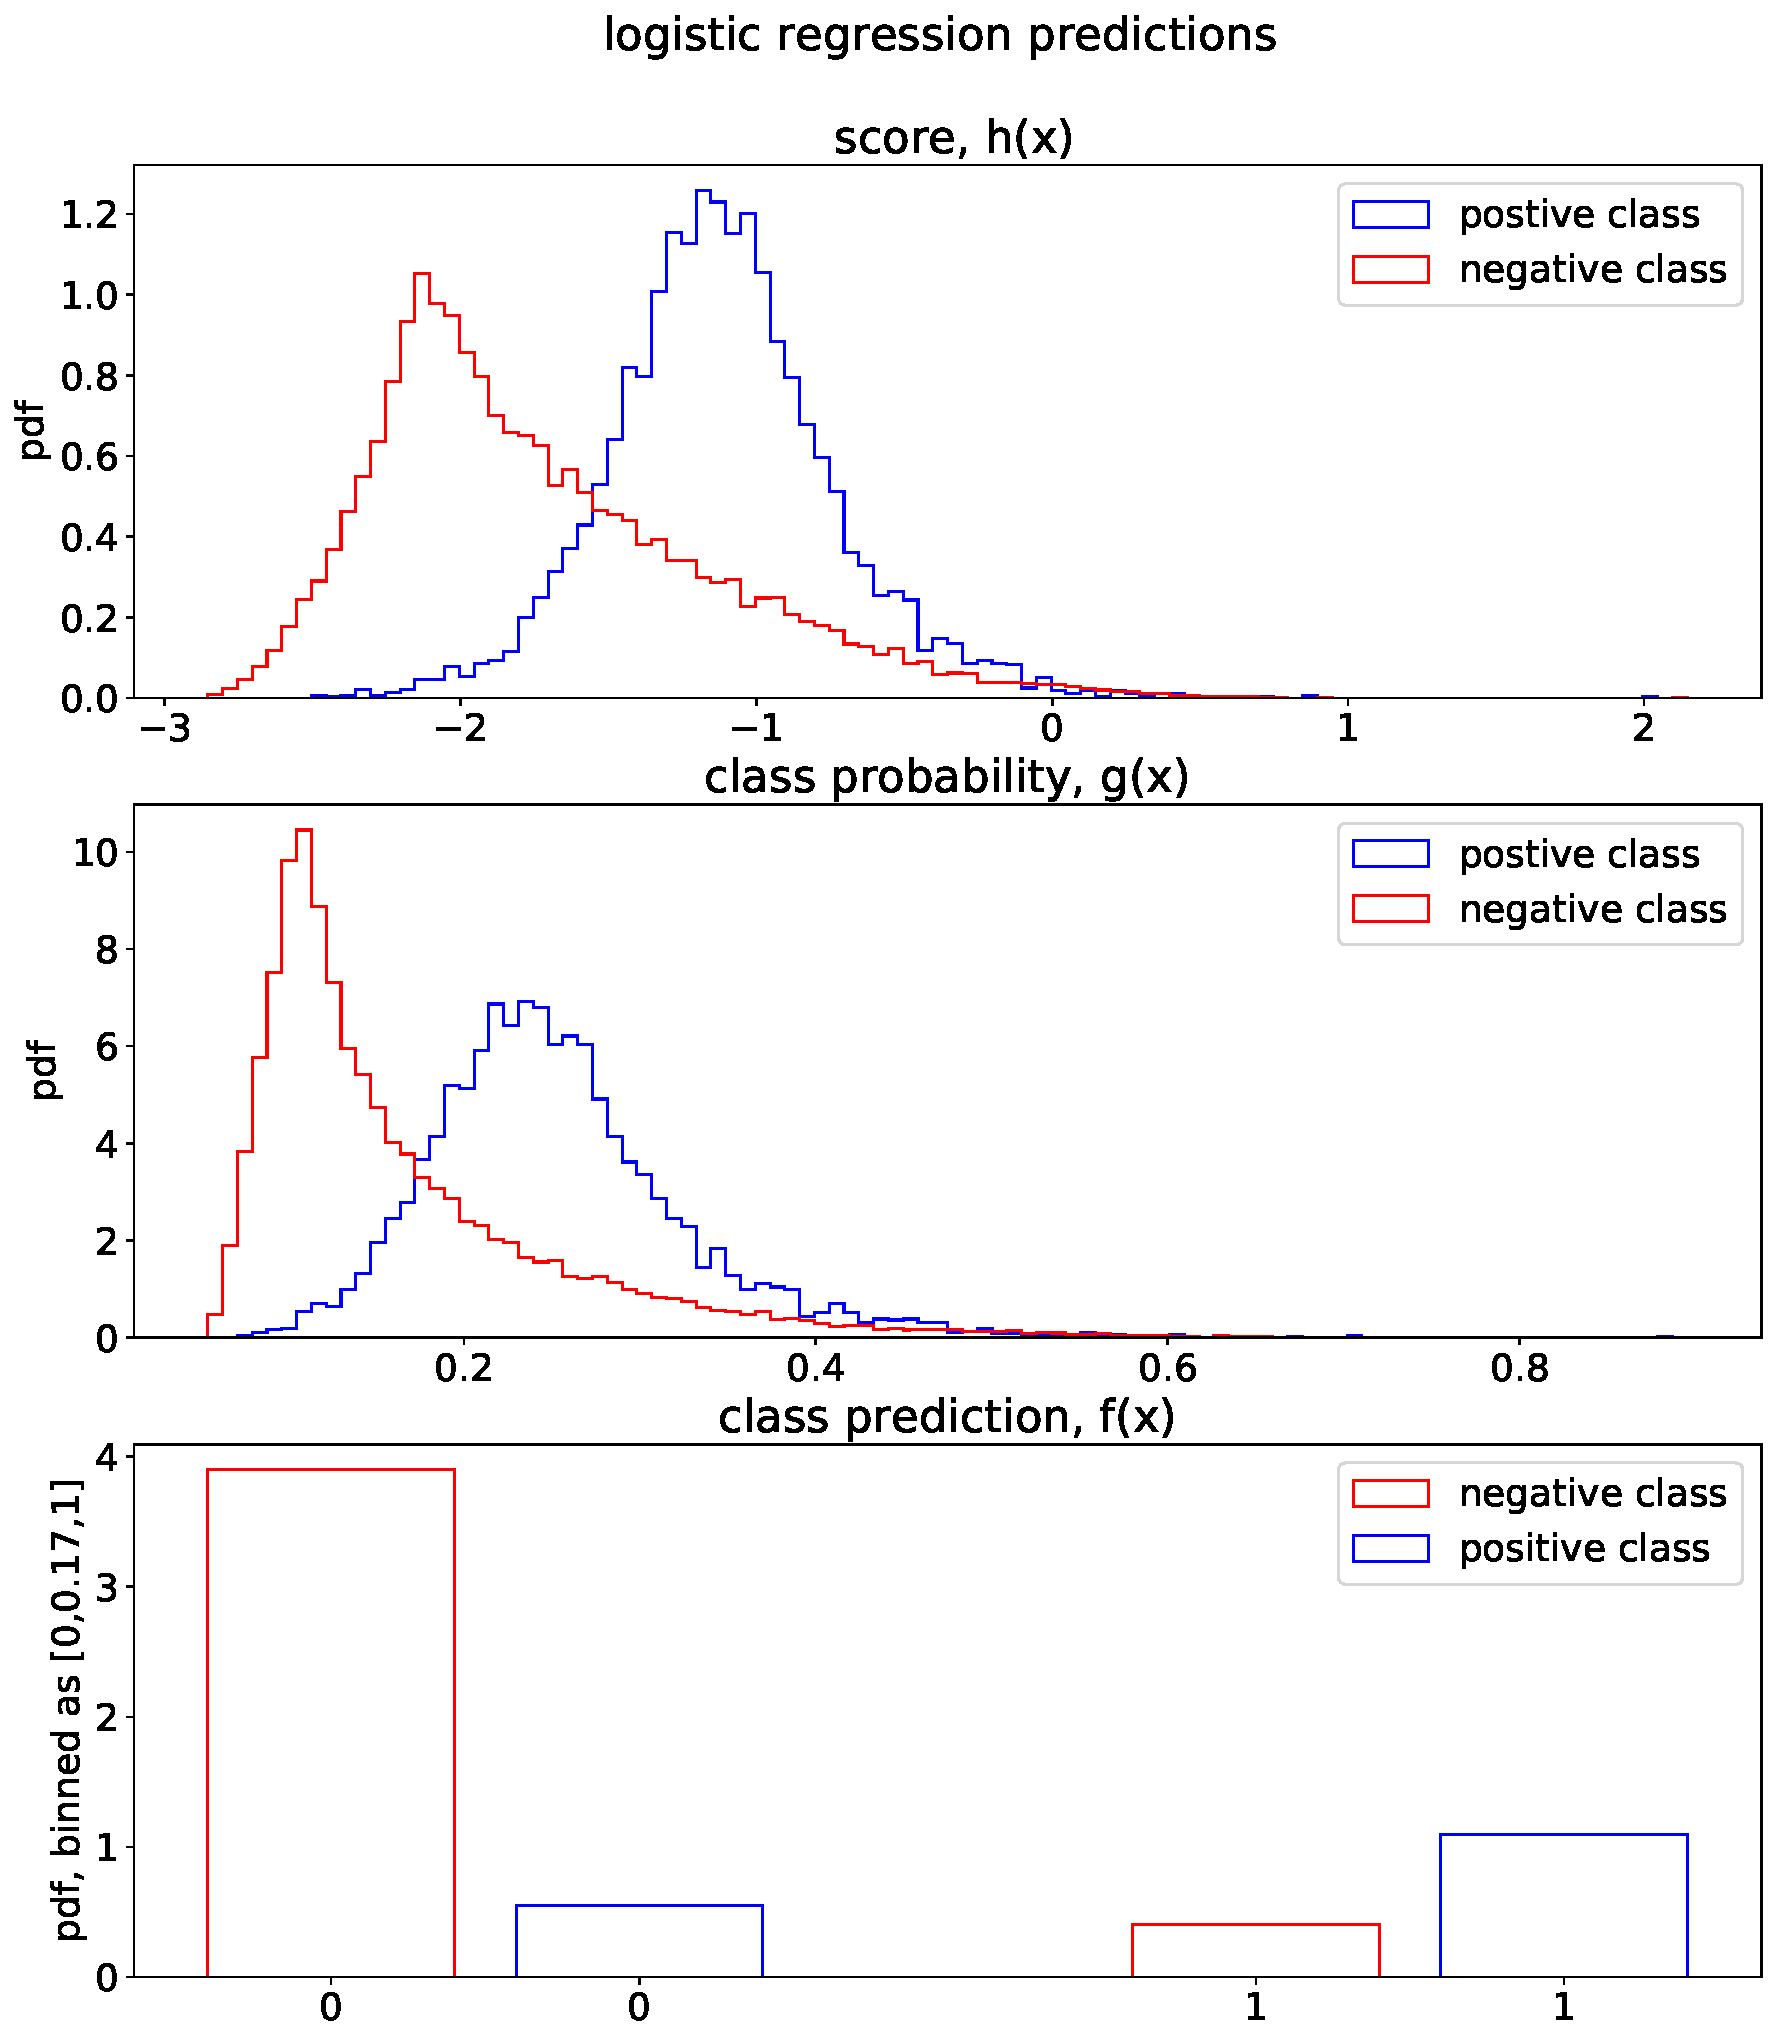
\includegraphics[width=\textwidth]{pics/torch_lr_predictions.pdf}
    \caption{Normalised distributions (pdf: probability density function) of the three scalar predictions of the pytorch logistic regression binary classifier using all features. The raw score from the linear combination of features, top; the class probability within $[0,1]$, middle; and the class (0 or 1) by deciding to split the classifier probabilities where the populations met at 0.17, bottom.}
    \label{fig:fghpredictions}
\end{figure}

\newpage
\subsection{Naive transitive partitioning using the classifier}
% explain how to get from log reg to object list
We now return to the motivating problem: how to determine physical objects from blobs on the sky. So far, we created a common catalogue of positional matches and successfully trained a classifier. As such, we'll set up the problem of finding physical objects as a task of telling which predicted positive matches are related to each other. Note that the classifier was not trained to perform this task. \\

We perform this relation task with what I call `naive transitive partitioning', breaking it down:
\begin{itemize}
    \item partitioning is dividing up the source catalogues into objects as subsets of related blobs, the partition must be total (everything is part of some object) and exclusive (nothing is part of more than one object)
    \item naive partitioning is performing this division purely based off of positional matching, this will divide up the physical sky into regions, each corresponding to a physical object
    \item naive transitive partitioning is relating any two positional matches if they share a source (e.g.\ $(T1,N1) \sim (T2,N1)$) or if there exists a chain of other related matches starting from one and ending at the other (e.g.\ $(T1,N1) \sim (T2,N1) \sim (T2,N2) \sim (T3,N2)$ implies that $(T1,N1) \sim (T3,N2)$), note the restriction that we only consider matches between TGSS to NVSS, so perhaps this should be called `naive transitive cross partitioning' as it'll miss objects composed solely of sources from one survey.
\end{itemize}
Performing this naive transitive partition over a small patch of sky we produce figure~\ref{fig:torch_lr_partition}, which shows all the internal TGSS to NVSS matches in each predicted object with the simple compact matches showing up as dots. In appendix~\ref{app:windows}, we display the same patch of sky in the cut-outs of TGSS and NVSS, see figure~\ref{fig:tgss-nvss-windows}. We also overlay a detail of the central, many-component object in figure~\ref{fig:torch_lr_partition} with the cut-out of TGSS, see figure~\ref{fig:overlay}. Clearly, we clearly the low precision, high recall of the classifier coupled with transitivity: lots of many-component objects, almost none of them real. In particular, the overlay shows the weakness of transitive partitioning, lots of close compact sources get all bundled together without checking their mutual matches.\\

Therefore, we conclude that naive transitive partitioning fails to identify real physical objects. Dropping transitivity is immediate, we should instead use something like checking that all pairs of sources in an object satisfy the classifier. However, even with a non-transitive partition, the thresholding problem of positional matching still remains for any naive partition: most separated sources are unrelated, but some related sources are very separated.

% torch_lr_partition, pretty snowflake picture
\begin{figure}[H]
    \centering
    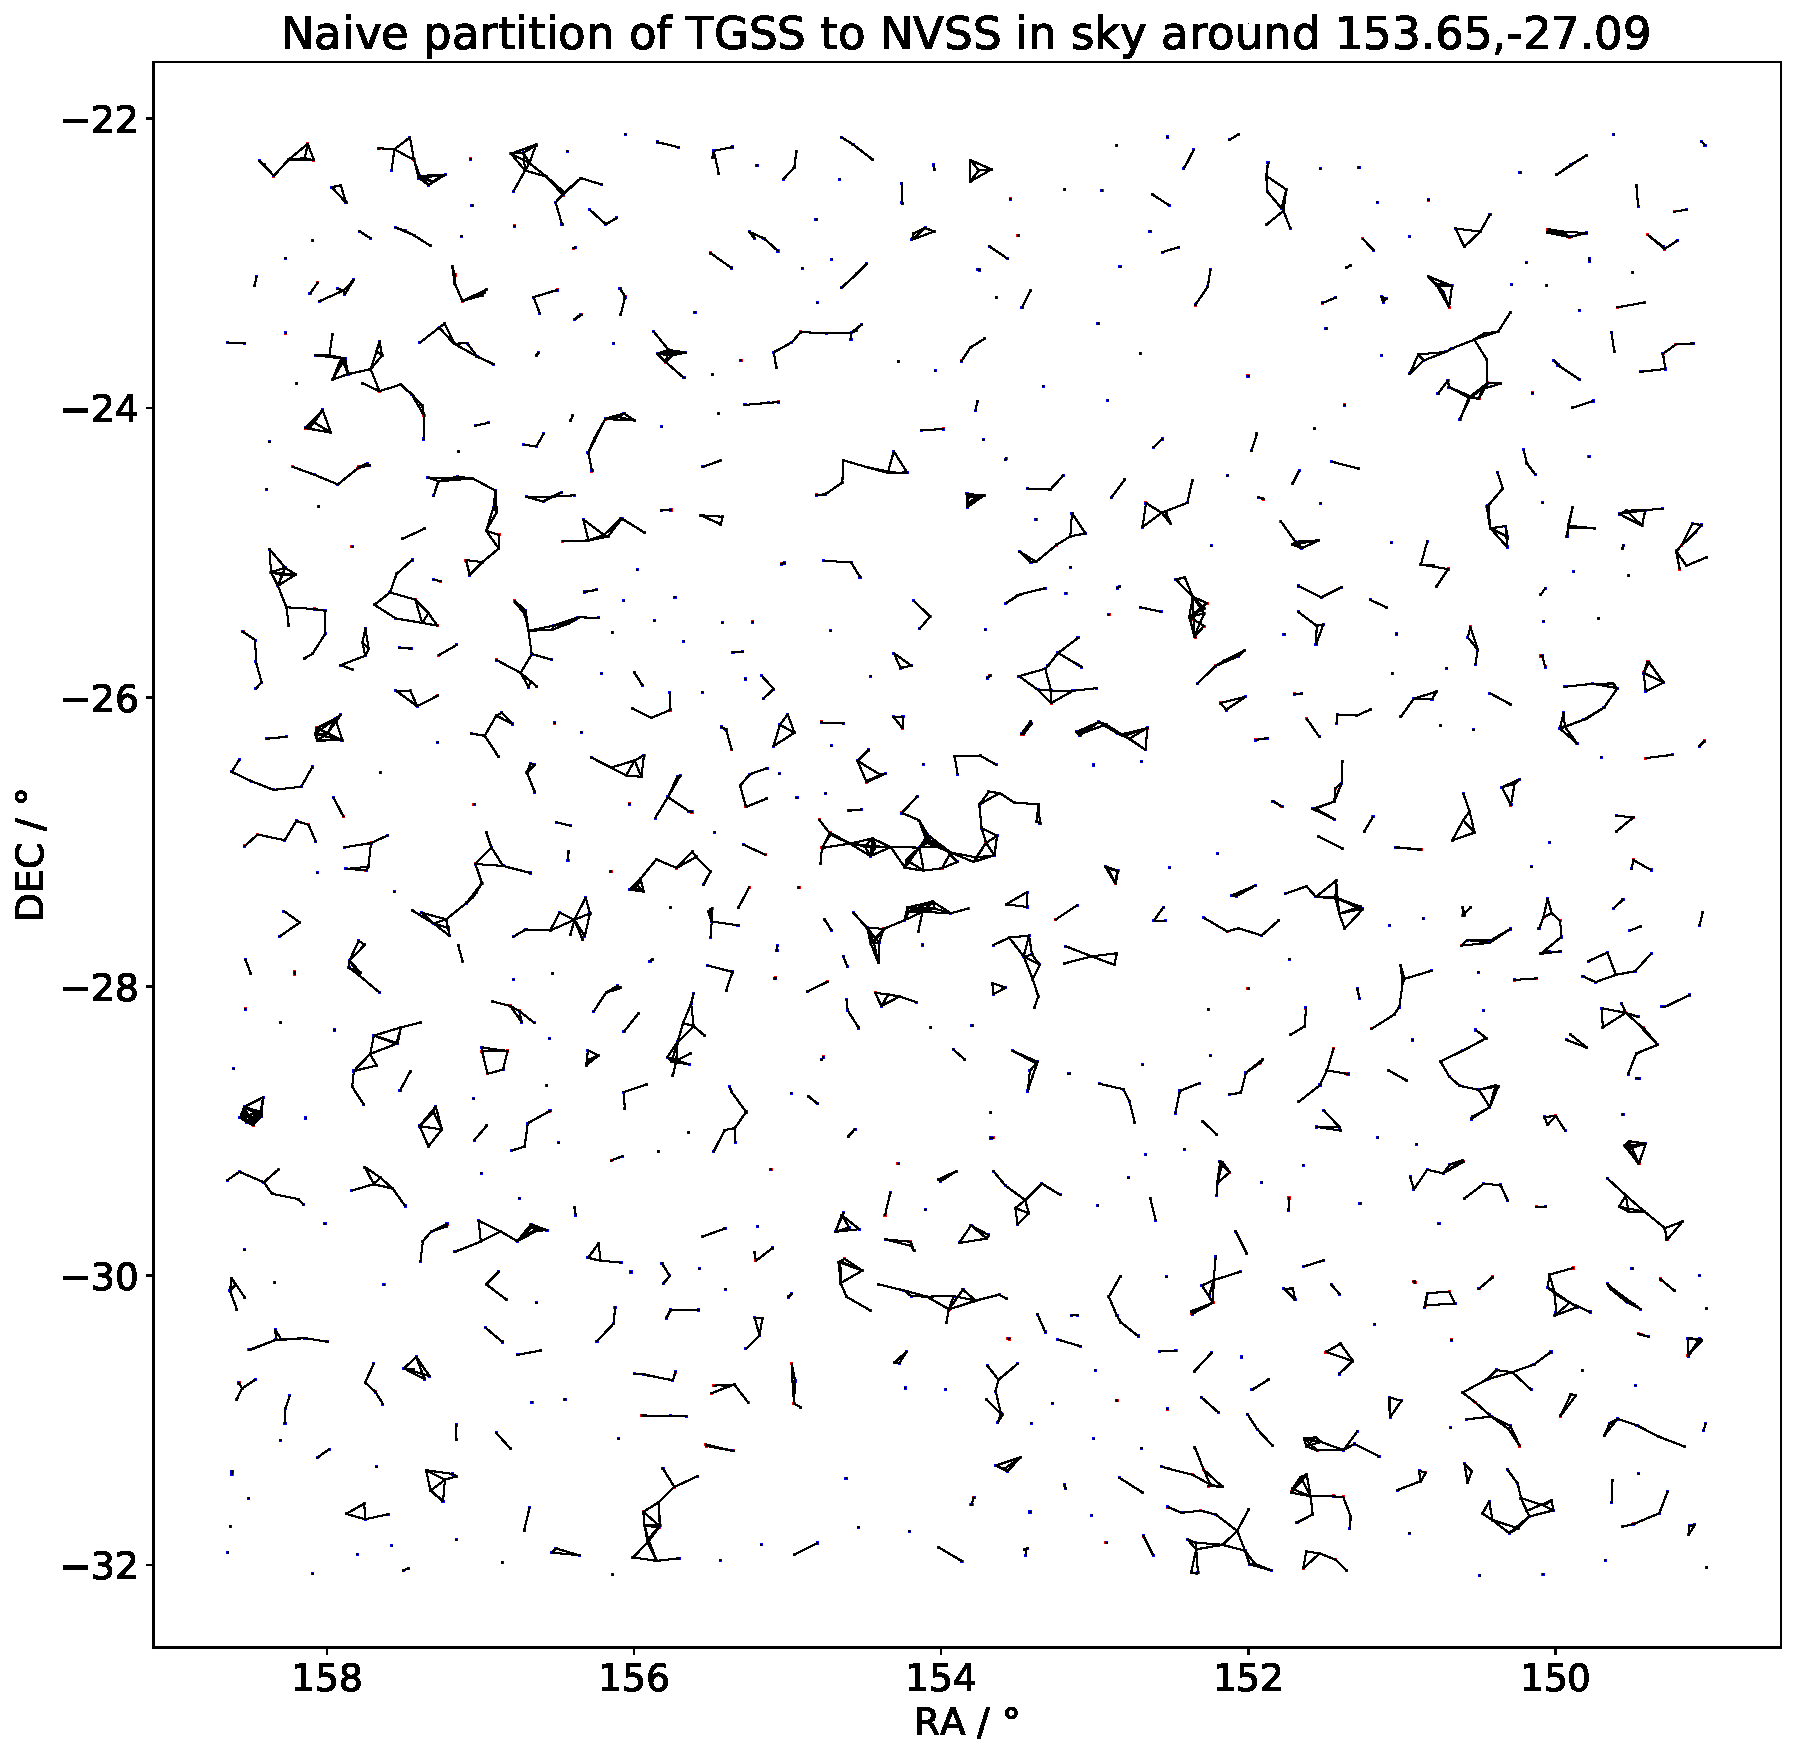
\includegraphics[width=\textwidth]{pics/torch_lr_partition.pdf}
    \caption{Naive transitive partition of the sky using classifier showing all TGSS (red points) to NVSS (blue points) matches within each object, note how this leads to large unphysical `constellations'.}
    \label{fig:torch_lr_partition}%snowflake
\end{figure}

\begin{figure}[H]
    \centering
    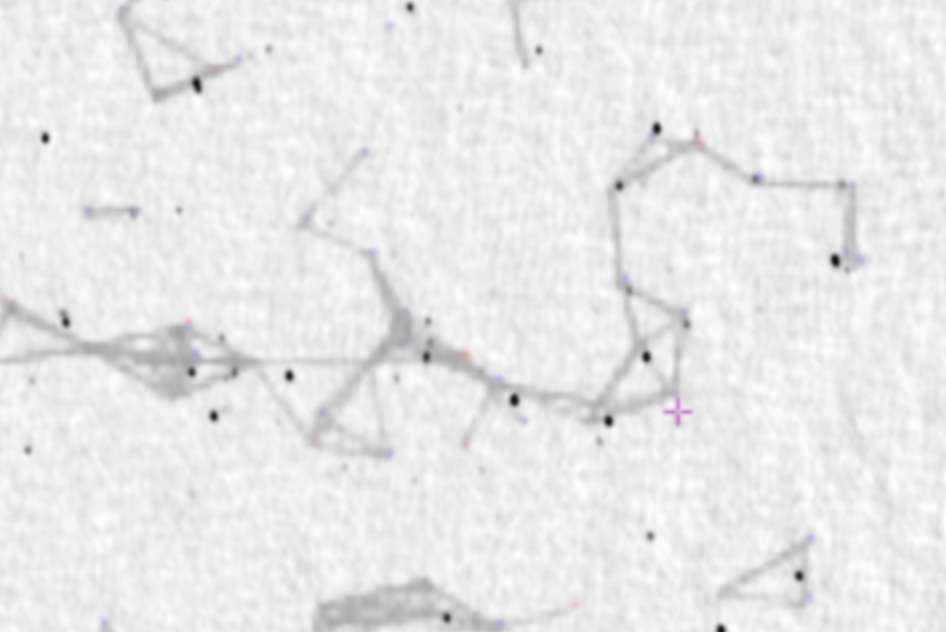
\includegraphics[width=0.6\textwidth]{pics/overlayoverlay.png}
    \caption{Overlay of central detail from figure~\ref{fig:torch_lr_partition} with TGSS cut-out. Not exactly aligned but one can clearly see that the naive transitive partition has linked distinct compact sources together into a many-component, non-existent physical object.}
    \label{fig:overlay}
\end{figure}

\section{Further discussion}
\label{sec:discussion}
Throughout this research, the unresolved issue is that positional matching cannot characterise all physical objects on the sky. Objects exist on the sky over scales of arcseconds to degrees and positional matching cannot handle this diversity. And any classifier trained against positional matching cannot produce a satisfying partition, because the positional matching labels themselves are not satisfying. This is true even if we fix the transitivity of the partition. For supervised machine learning, this, challenging the labels, is the critical attack one can make. We did present the classifier with a set of manual labels to test against, but these were not decisive enough and were limited to come from a common catalogue of loosely positional matched sources. For the worst case, degree sized objects, the classifier was never trained or tested against, but would have failed.\\

% wild speculation
So what could be done, if we are to wildly speculate? The first thing would be to return to the manual labels and create them anew for objects across the size scale. Then instead of testing, train the classifier against this small set of manual labels, with some strong regulariser as to not overfit the limited data. This would require a catalogue of matches out to a separation limit in degrees. Also, consider selecting a different model than logistic regression, one non-linear and with decision capabilities (e.g.\ a layered network). The common thread with positional matching and the spectral index is that they are both very strong at excluding extreme cases, and both poor at making decisions in fuzzy regimes, so use them in the first step of the decision tree to filter. One could also imagine then that the gaussian and positional angle alignment features could then become relevant. As is, we can't take any more features from the raw source catalogues (except for fixing positional angle as mentioned in \ref{sec:catalogue_of_matches}, and properly correcting for beam sizes). But we could move one layer back and take feature vectors as the radio cut-outs, as the raw photometric data itself.\\

There's also consideration for not approaching the problem as binary classification. Our manual labels could instead be known objects as a list of sources. And the classifier could then take a single source and predict the likelihood that falls into various different partitions. The key is that cross-identification does not seem unsolvable, we just need to update our approach.

\bigskip
\subsection{Conclusions}
Our goal was to cross-identify TGSS and NVSS as to be able to identify the real, physical objects in the sky. To this end, we constructed a common catalogue of positional matches of TGSS to NVSS sources within $\ang{;2;}$ over the shared sky and successfully reproduced the initial results of \citet{posmatchpaper}.\\

We then restated the problem as a binary classification task and trained a logistic regression classifier against positional matching labels. This classifier successfully predicted positional matching and manual labels, both with and without the separation feature.\\

Finally, we used the classifier to perform a naive transitive partition of the sky into predicted physical objects. This partition did not appear remotely physical. We find the fault to lie with naive transitive partitioning and positional matching itself.

\bigskip
\nocite{*}
\bibliographystyle{plainnat}
\bibliography{refs}
% - - - - - - - - - - - - - - - - - - - - - - - - - - - -

\newpage
\section{Appendices}
\subsection{Artefact README.txt excerpt}
\label{app:artefact}
Current build found at:
\url{https://github.com/MatthewJA/blobmatch}

TGSS and NVSS radio object surveys available from:\\
\url{https://github.com/MatthewJA/blobmatch/releases/download/v0.1/TGSSADR1_7sigma_catalog.tsv.gz}\\
\url{https://github.com/MatthewJA/blobmatch/releases/download/v0.1/CATALOG.FIT.gz}

\begin{verbatim}
Directory structure:
blobmatch/
    source/
        (all .ipynb notebooks, manual_labels.csv)
    report/
        pics/
            (all plots as .pdf saved by above
            notebooks, also cut-out comparison)
        main.tex
        report.pdf
    project/
        (non-plot outputs of notebooks except
        sky_matches.csv and sky_catalogue.csv,
        also defunct scipts and plots)
    README.txt
    LICENSE
    .gitignore
\end{verbatim}

blobmatch/source/ .ipynb notebooks:
\begin{itemize}
    \item feature\_vectors.ipynb\\
(constructs feature vectors from source catalogues in a patch, labels based off of positional matching)

    \item torch\_logistic\_regression.ipynb\\
(performs logistic regression using pytorch, partitions sky into physical objects)

    \item sklearn\_logistic\_regression.ipynb\\
(performs logistic regression and random forest using sklearn)

    \item score\_feature\_vectors.ipynb\\
(scores the match feature vectors in patch against various metrics, finds each individual source's best match)

    \item sky\_positional\_matching.ipynb\\
(constructs catalogue of primitive feature vectors over entire sky in catalogues, performs positional matching)
\end{itemize}

\subsection{Explicit scorers}
\label{app:scorers}
During research, we also created some other explicit score functions along with the separation scorer. Variations included: checking if a match was in the catalogue, using the spectral index histogram as a probability density function (pdf), and weighted combinations thereof against the separation score. These hand-made score functions did not produce nice results and were left behind for logistic regression. Figure~\ref{fig:spectral_scorer} shows the scorer that used the spectral index distribution in figure~\ref{fig:hist_alpha_comparison} as a probability distribution. Although this sounded good, the disjoint results it produced (perhaps for binning reasons) are undesirable. Note that score distribution shown is over the patch, while the spectral index pdf was over the entire sky. Also, since it outputs within $[0,1]$ to stay consistent with our three types of predictors, this is not a score but a probability.
\begin{figure}[H]
    \centering
    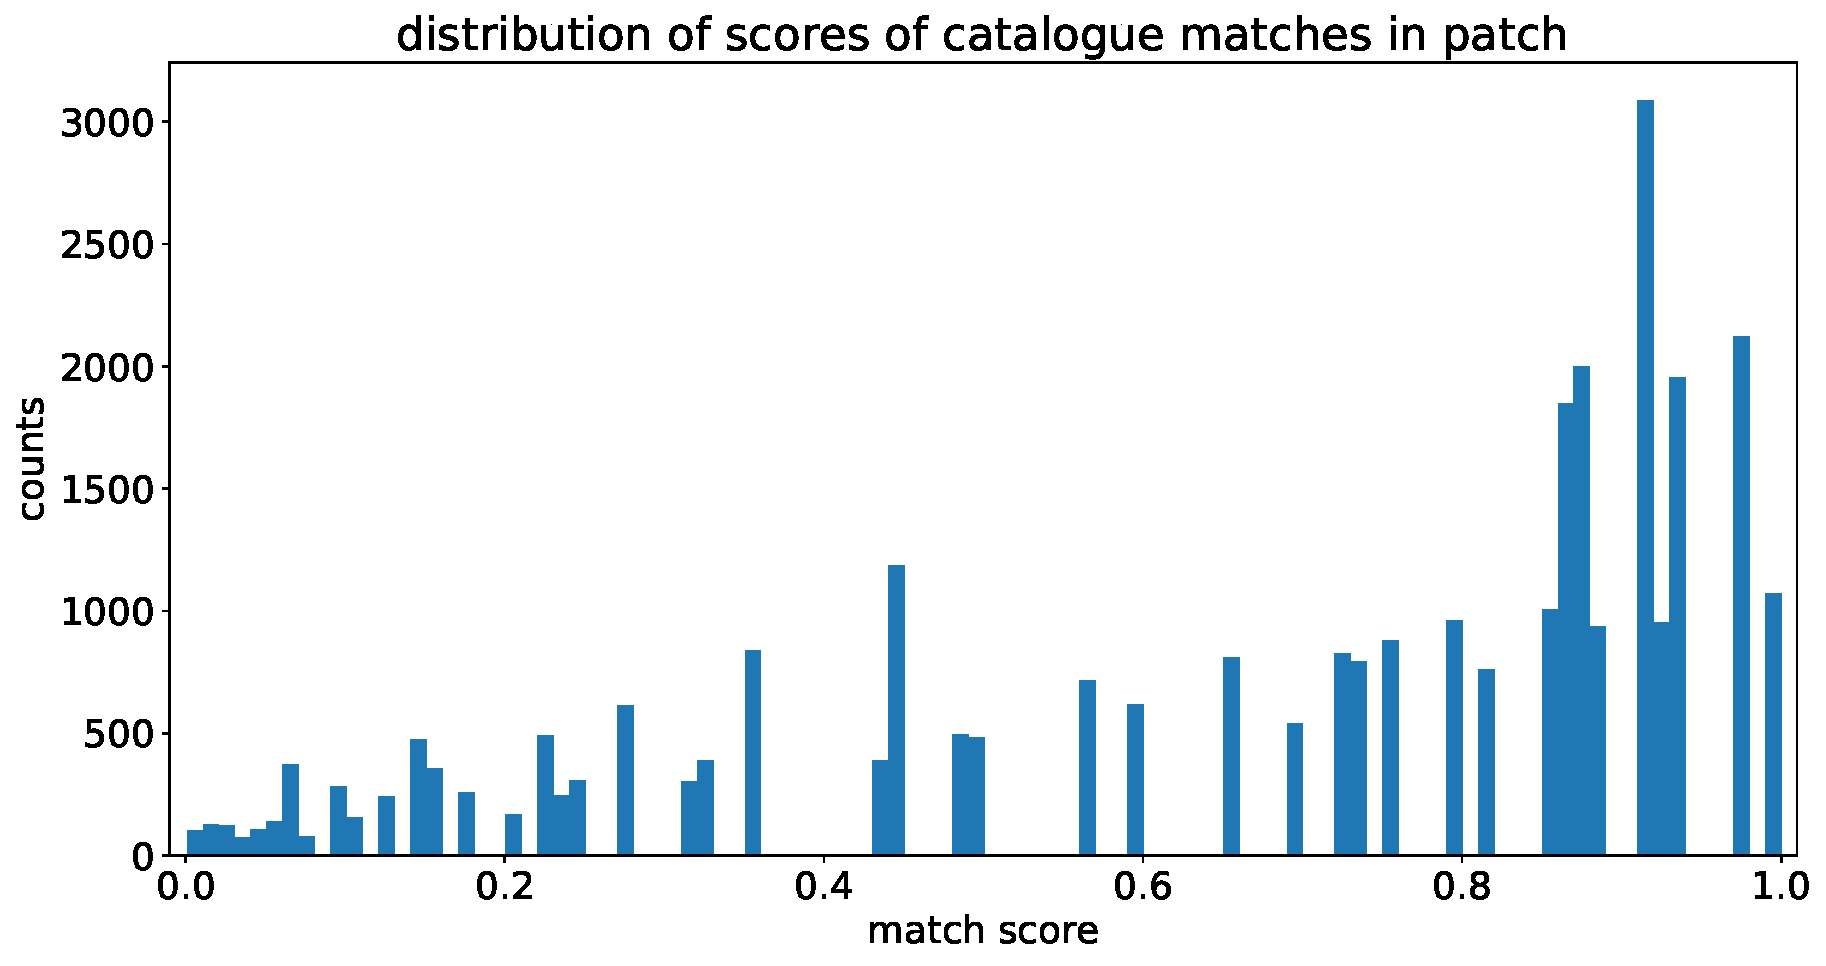
\includegraphics[width=\textwidth]{pics/hist_patch_cat_score_spectral.pdf}
    \caption{Distribution of probabilities from explicit scorer that uses the spectral index distribution as a pdf.}
    \label{fig:spectral_scorer}
\end{figure}

\subsection{Loss curve}
\label{app:losses}
% torch_lr_losses_nosep
\begin{figure}[H]
    \centering
    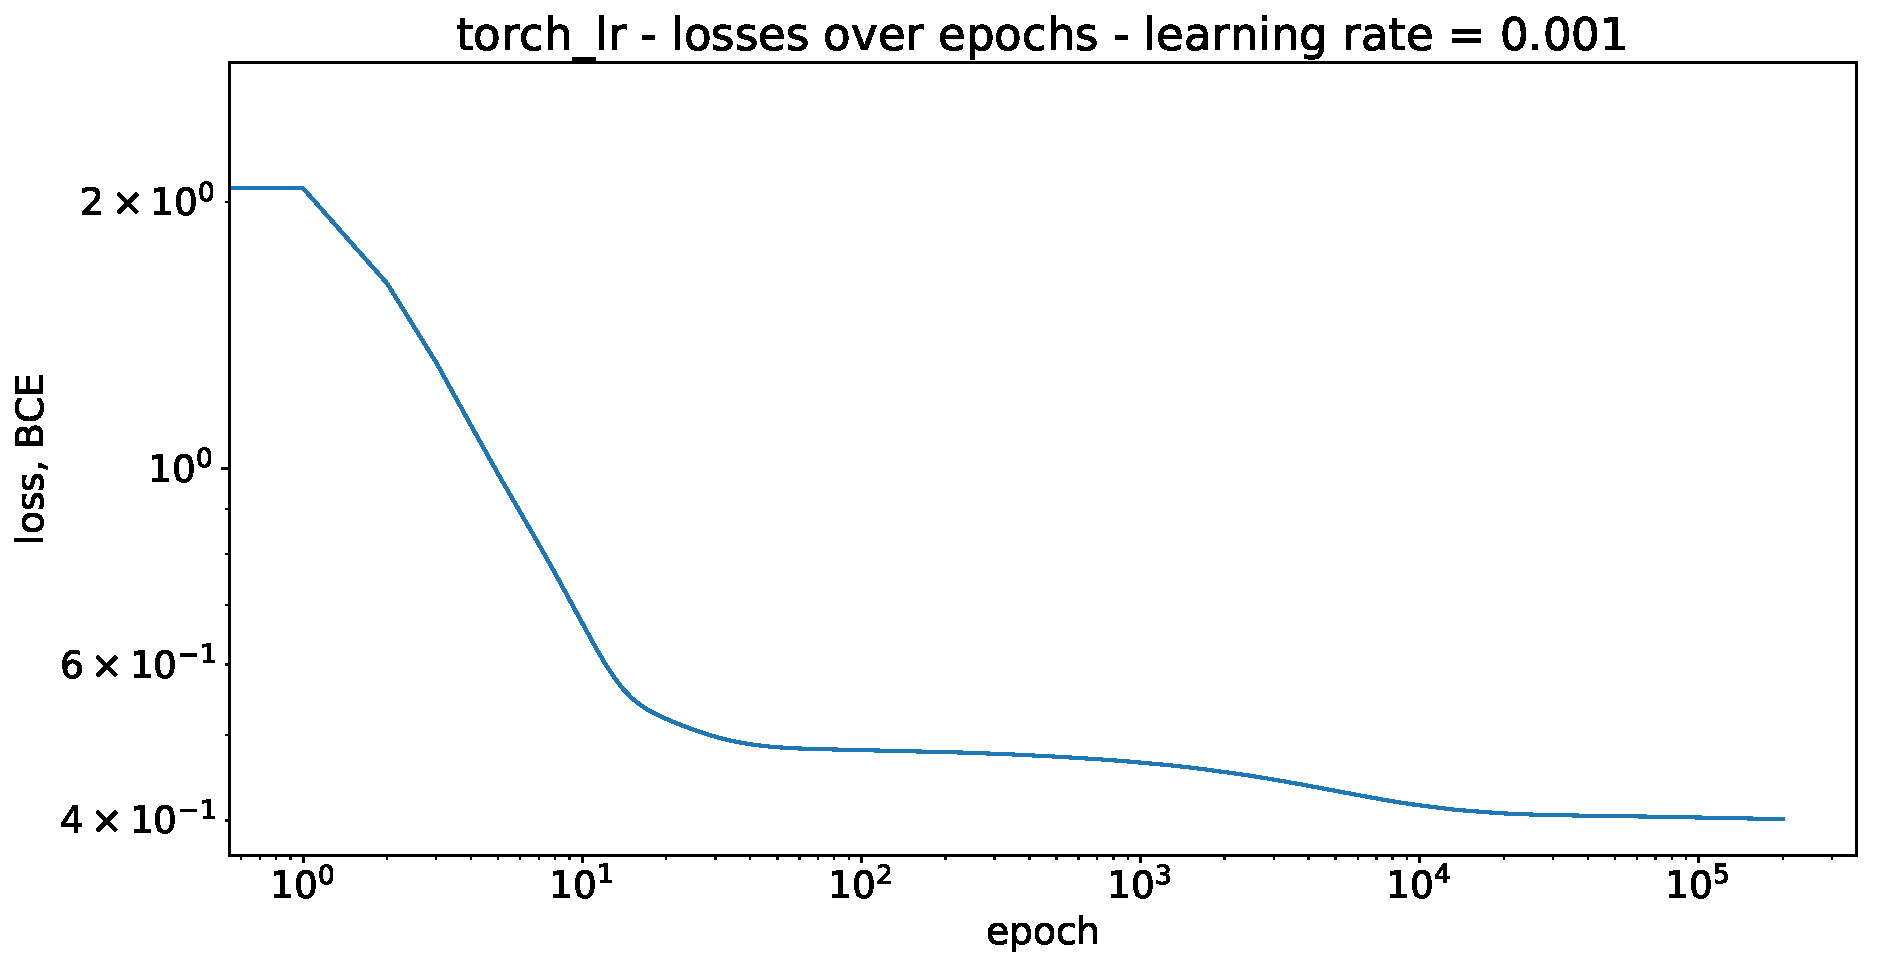
\includegraphics[width=\textwidth]{pics/torch_lr_losses_nosep.pdf}
    \caption{Loss curve for pytorch logistic regression for model without separation, note the decent and then stabilisation after 1e5 epochs of training, we can be hopeful that we've reached some local minimum.}
    \label{fig:torch_lr_losses_nosep}
\end{figure}

\newpage
\subsection{Scikit-learn}
\label{app:sklearn}

We also ran logistic regression through scikit-learn~\citep{sklearn}, this proved both faster and more accurate than the pytorch model. See table~\ref{tab:accuracy} for accuracy. The improvement in accuracy may be due to regularisation.

% sklearn_lr
\begin{figure}[H]
    \centering
    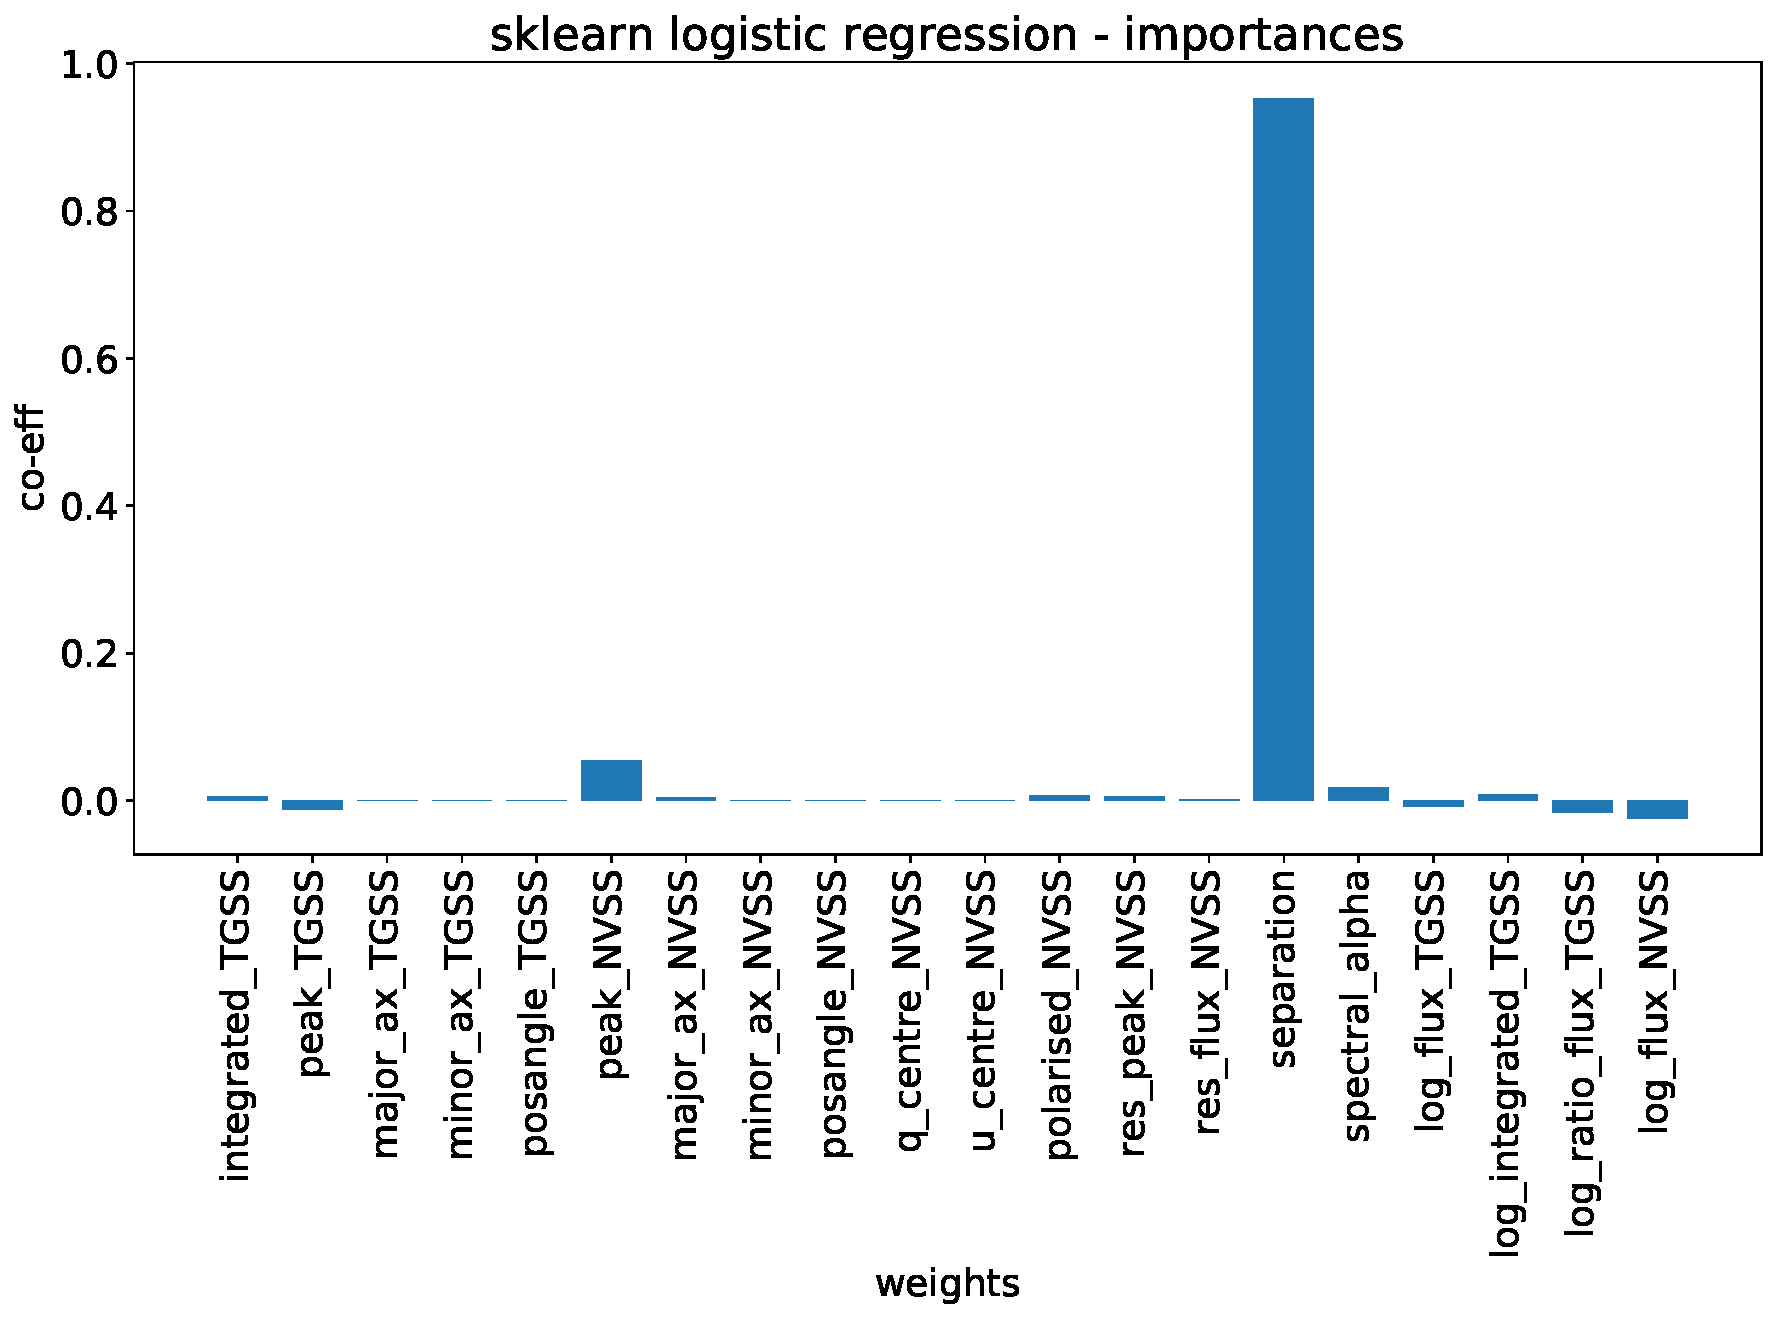
\includegraphics[width=\textwidth]{pics/sklearn_lr.pdf}
    \caption{Weights (or rather, importances) from scikit-learn logistic regression model after training.}
    \label{fig:sklearn_lr}
\end{figure}

\subsection{TGSS-NVSS view on partition}
\label{app:windows}

% tgss_window, nvss_window
\begin{figure}[H]
    \begin{subfigure}{1\textwidth}
        \centering
        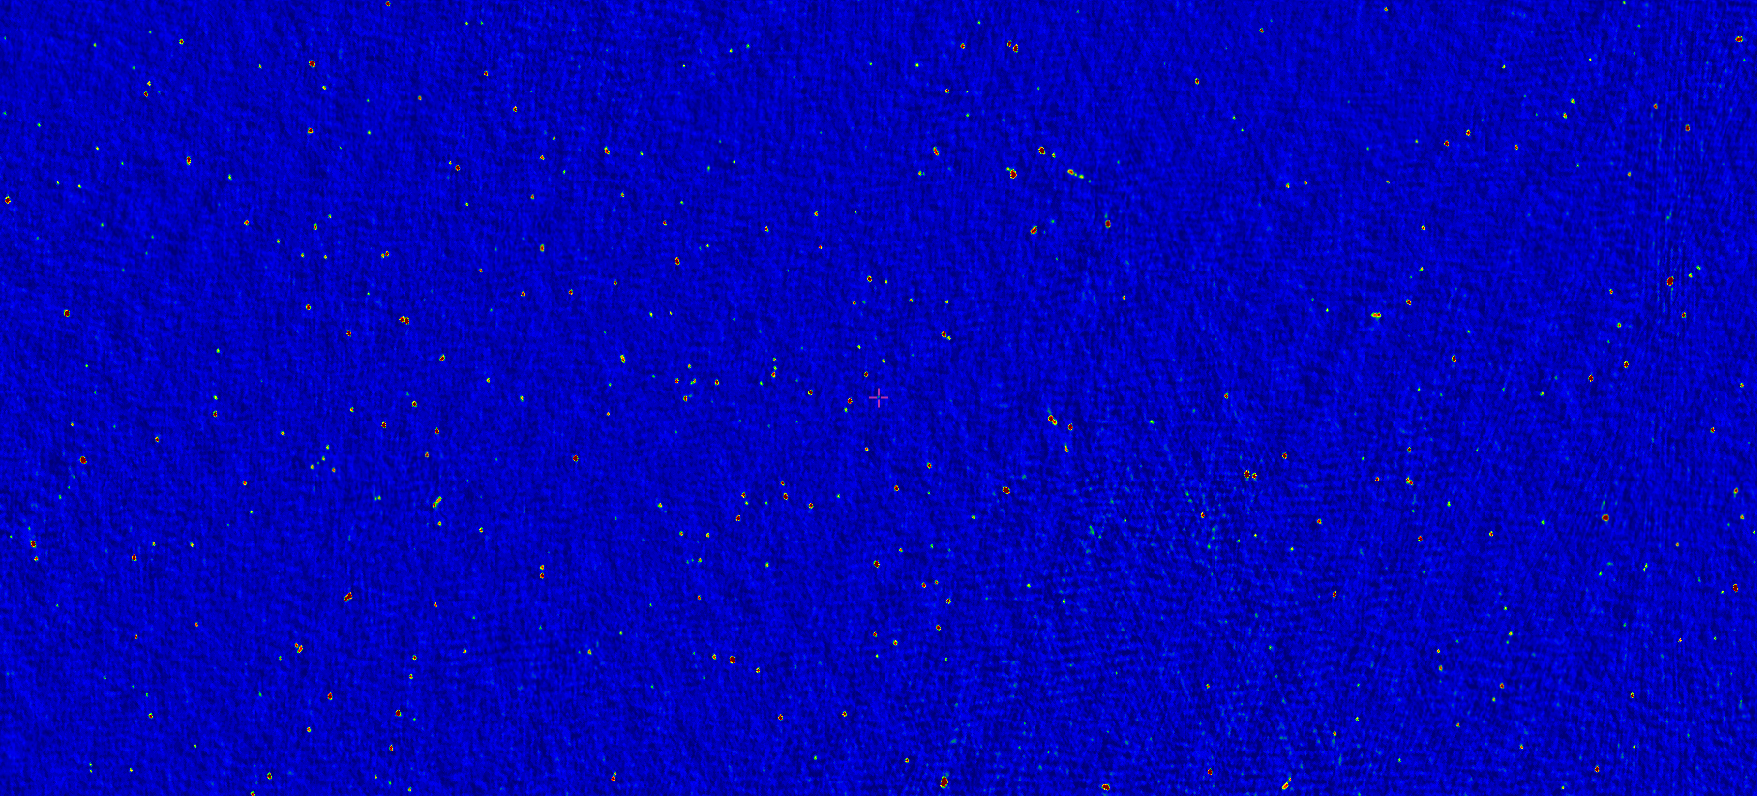
\includegraphics[width=1\linewidth]{pics/tgss_window.pdf}
        % \caption{Put your sub-caption here}
    \end{subfigure}
    \\
    \begin{subfigure}{1\textwidth}
      \centering
        % include second image
        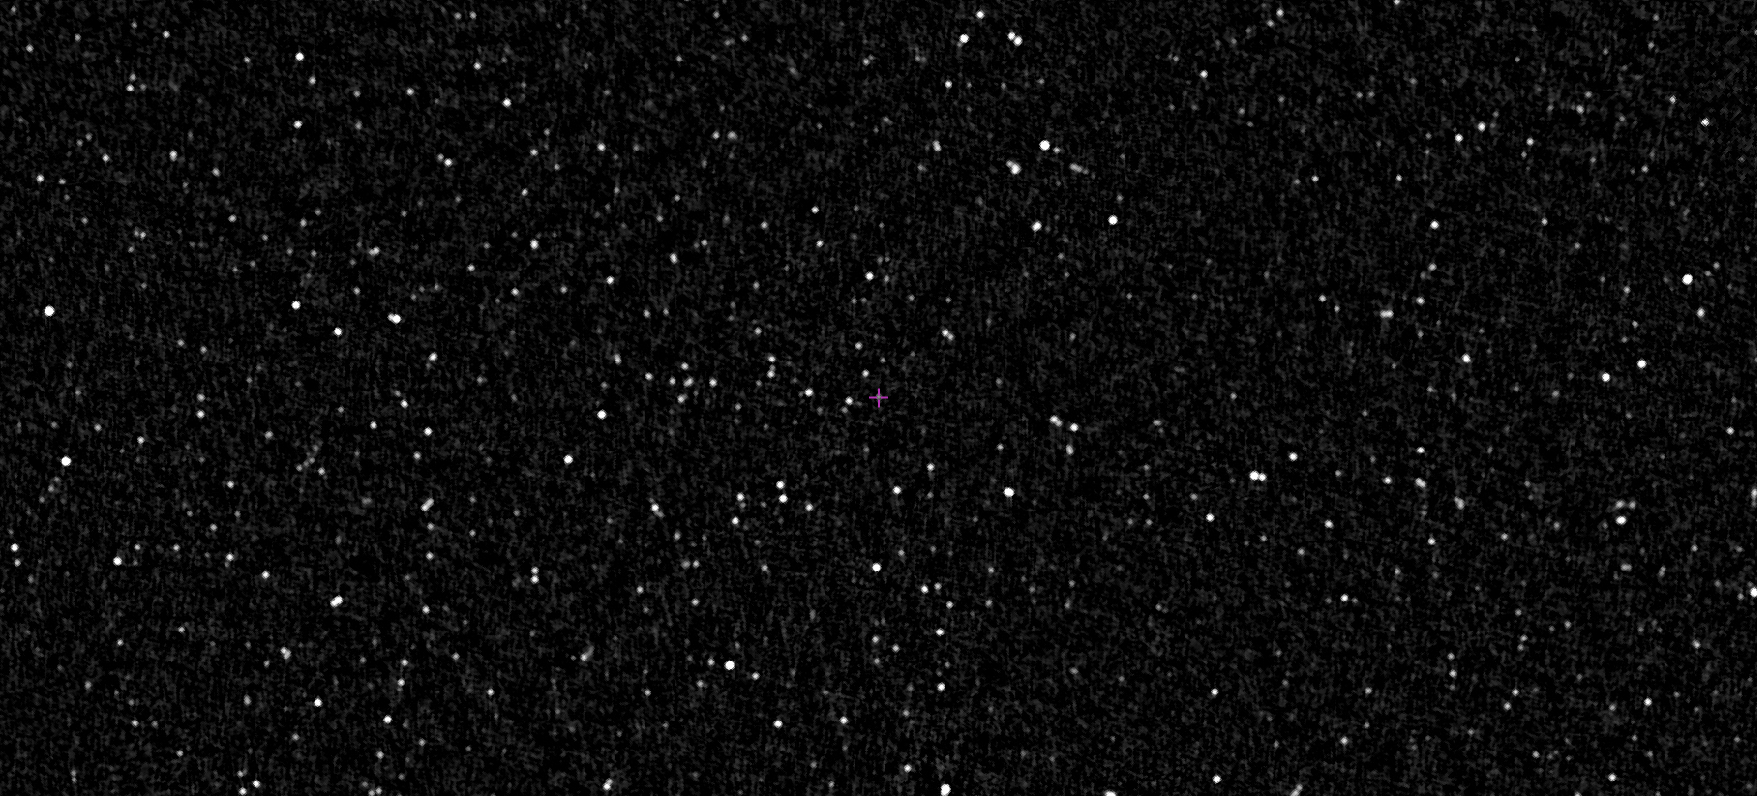
\includegraphics[width=1\linewidth]{pics/nvss_window.pdf}
        % \caption{Put your sub-caption here}
    \end{subfigure}
    \caption{Cut-outs of TGSS and NVSS over the partitioned patch of sky shown in
    figure~\ref{fig:torch_lr_partition}, taken from AladinLite~\citep{aladinlite} in 5 degree window around  J101436.8-270532.}
    \label{fig:tgss-nvss-windows}
\end{figure}


\end{document}
% - - - - - - - - - - - - - - - - - - - - 
